% This is our submission, modified from:
% the file JFP2egui.lhs
% release v1.02, 27th September 2001
%   (based on JFPguide.lhs v1.11 for LaLhs 2.09)
% Copyright (C) 2001 Cambridge University Press

\NeedsTeXFormat{LaTeX2e}

\documentclass{jfp1}

%%% Macros for the guide only %%%
%\providecommand\AMSLaTeX{AMS\,\LaTeX}
%\newcommand\eg{\emph{e.g.}\ }
%\newcommand\etc{\emph{etc.}}
%\newcommand\bcmdtab{\noindent\bgroup\tabcolsep=0pt%
%  \begin{tabular}{@{}p{10pc}@{}p{20pc}@{}}}
%\newcommand\ecmdtab{\end{tabular}\egroup}
%\newcommand\rch[1]{$\longrightarrow\rlap{$#1$}$\hspace{1em}}
%\newcommand\lra{\ensuremath{\quad\longrightarrow\quad}}

\jdate{August 2017}
\pubyear{2017}
\pagerange{\pageref{firstpage}--\pageref{lastpage}}
\doi{...}

%\newtheorem{lemma}{Lemma}[section]

\newcommand{\pipe}{|}
\usepackage{tikz}

\usepackage{filecontents}
\usepackage{pgfplots, pgfplotstable}
\usepgfplotslibrary{statistics}

\usepackage[T1]{fontenc}
\usepackage[utf8]{inputenc}

\usepackage{tablefootnote}

%\usepackage{color}
\usepackage{hyperref}

%\usepackage{subcaption}

\usepackage[round,sectionbib]{natbib}
%% https://tex.stackexchange.com/questions/148992/changing-the-heading-style-of-references-section
%% and jfp1.cls
\renewcommand\refname{References}
\makeatletter
\renewcommand\bibsection{%
  \section*{\refname}%
}%
\makeatother

\usepackage{csquotes}

% \usepackage{placeins} %% unneeded

\usepackage{microtype}
\DisableLigatures[>,<]{encoding = T1,family=tt*} 

% für Listings
%\usepackage{listings}


\renewcommand{\cite}[1]{\citep{#1}}

\newcommand{\citHughes}{\citep{HughesArrows}}

%\newcommand{\inlinecode}[1]{\texttt{#1}}
\newcommand{\inlinecode}[1]{\emph{#1}} %%% booo
%%% |code| is inline code in lhs2tex

%\newcommand{\fixme}[1]{\colorbox{red}{#1}}

%%%%%% more fun and typography

\usepackage{xifthen}

\newboolean{anonymous}
\setboolean{anonymous}{False}

\usepackage[british]{babel}

\usepackage{siunitx}

%%\usepackage{tipa} %% causes problems with lhs2tex?!

\usepackage{xspace}
\usepackage{xcolor}
\newcommand{\hl}[1]{\textcolor{red}{#1}}
\newcommand{\comm}[2]{\textcolor{red}{\bfseries #1: #2}}
%\newcommand{\comm}[2]{}
\newcommand{\olcomment}[1]{\comm{OL}{#1}}
\newcommand{\mbcomment}[1]{\comm{MB}{#1}}
\newcommand{\ptcomment}[1]{\comm{Phil}{#1}}
%\newcommand{\done}{\xspace\hl{done!}\xspace}
\newcommand{\fixme}{\mbcomment}

\DeclareRobustCommand{\xth}{\textsuperscript{th}\xspace}
\DeclareRobustCommand{\st}{\textsuperscript{st}\xspace}
\DeclareRobustCommand{\nd}{\textsuperscript{nd}\xspace}
\DeclareRobustCommand{\xrd}{\textsuperscript{rd}\xspace}

%% kuerzel
%\newcommand{\todo}{\textcolor{red}{\bfseries TODO!}\xspace}
\newcommand{\done}{\textcolor{green}{\bfseries done!}\xspace}
\DeclareRobustCommand{\hairspn}{\hspace{1pt}\nolinebreak}% hair space with no break

% \DeclareRobustCommand{\ie}{{i.\hairspn{}e.\nopagebreak[4] }}
% \DeclareRobustCommand{\eg}{{e.\hairspn{}g.\nopagebreak[4] }}
% \DeclareRobustCommand{\fe}{{f.\hairspn{}e.,}\nopagebreak[4] }
\DeclareRobustCommand{\ie}{{i.\hairspn{}e.~}}
\DeclareRobustCommand{\eg}{{e.\hairspn{}g.~}}
\DeclareRobustCommand{\fe}{{f.\hairspn{}e.,~}}
\DeclareRobustCommand{\ad}{{A.\hairspn{}D.\xspace}}
\DeclareRobustCommand{\bcc}{{A.\hairspn{}C.\xspace}}
\DeclareRobustCommand{\wrt}{w.\hairspn{}r.\hairspn{}t.~}
\DeclareRobustCommand{\etc}{etc.\ }
\DeclareRobustCommand{\cf}{\textit{cf.~}}
\DeclareRobustCommand{\viz}{\textit{viz.~}}
%\DeclareRobustCommand{\hof}{higher-or\-der function\xspace}

% %% the numberings
\DeclareRobustCommand{\xth}{\textsuperscript{th}\xspace}
\DeclareRobustCommand{\st}{\textsuperscript{st}\xspace}
\DeclareRobustCommand{\nd}{\textsuperscript{nd}\xspace}
\DeclareRobustCommand{\xrd}{\textsuperscript{rd}\xspace}

\newcommand{\tabsepbakup}{\tabcolsep}
%% for narrower tables

%% nice tables
\usepackage{booktabs}
%\usepackage{multirow}

%% more microtype
\microtypecontext{spacing=nonfrench} %% log said so

\usepackage{subfig}


%% fight for pipepipepipe
\newcommand{\pipepipepipe}{\ensuremath{\mathbin{\mid\!\mid\!\mid}}\xspace}
%%% ^^^^ keep consistent with definition at the top of main.lhs
%%%\newcommand{\pipepipepipe}{\inlinecode{|||}\xspace}

%%% JFP requirements:
%%% Harvard citing style, "(Curry 1933)".
%%% code: identifies italic, keywords bold
%%% figures: eps(!) or ps (can convert pdf), eventually provide a greyscale version, color NOT in cmyk



\title{Arrows for Parallel Computations}
\ifthenelse{\boolean{anonymous}}{%
\author{Submission ID xxxxxx}
}{%
%\author{Martin Braun, Phil Trinder, and Oleg Lobachev}
%\affiliation{University Bayreuth, Germany and Glasgow University, UK}
 \author[M. Braun, P. Trinder, and O. Lobachev]%
        {MARTIN BRAUN\\
         University Bayreuth, 95440 Bayreuth, Germany\\
         PHIL TRINDER\\
		 Glasgow University, Glasgow, G12 8QQ, Scotland\\
		 \and\ OLEG LOBACHEV\\
		 University Bayreuth, 95440 Bayreuth, Germany}
}% end ifthenelse



\begin{document}

\label{firstpage}

\def\SymbReg{\textsuperscript{\textregistered}}

\maketitle

%% environment inside
\begin{abstract}
Arrows were introduced in John Hughes paper as a general interface for computation and therefore as an alternative to monads for API design \citHughes. In the paper Hughes describes how arrows are a generalization of monads and how they are not as restrictive. In this paper we will use this concept to express parallelism.
\\\\
First, we give an introduction to some of the possible ways to add parallelism to Haskell programs. Then, we give the basic definition of Arrows, which is followed up by the introduction of some utility functions used in this paper. Next, we introduce the \code{ArrowParallel} typeclass together with backends for it written with the parallel Haskells introduced earlier, finishing up with the benefits of this new way of writing parallel programs. After this we give the definition of several parallel skeletons. Then, we introduce some syntactic sugar to mimic the sequential arrow combinators introduced by Hughes \citHughes ~but with parallelism added. We also give benchmarks of our newly created parallel Haskell. Finally we give a short conclusion of what we managed to achieve.
\end{abstract}

\tableofcontents

	%
	%%include abstract.lhs
	%
	%\newpage
	\tableofcontents
	%\pagebreak
	%\section{Motivation}
%Arrows were introduced in John Hughes paper as a general interface for computation and therefore as an alternative to Monads for API design \citHughes. In the paper Hughes describes how arrows are a generalization of Monads and how they are not as restrictive. In this paper we will use this concept to express parallelism.

\section{Introduction}
\label{sec:introduction}
% \olcomment{todo, reuse 5.5, and more}
%
% \mbcomment{
% Haskell is Spielwiese für Parallelität; verschiedene Ansätze (Par, Multicore, Eden); Orthogonale Ansätze; Verwenden höchstens eine Monade - manchmal auch nur intern; Wir wollen Parallelität mit Arrows abbilden, was noch niemand gemacht hat;
% Statt einer eigenen Implementierung definieren wir ein "shallow embedded DSL" (ACHTUNG, ist das der richtige Name? effektiv API);
% Umsetzung mit verschiedenen parallelen Haskells; We tame the zoo of parallel Haskells und vergewissern uns dass es nicht viel Overhead bringt
% }
%
% blablabla arrows, parallel, haskell.
%
% \olcomment{An attempt ---->}
%%%%%

One particular reason for this is the ease of introducing new sophisticated language
concepts. Parallel functional languages have a long history of being used for experimenting with novel parallel programming paradigms including the expression of parallelism. Haskell, which we focus on in this paper, has  several mature implementations. We regard here in-depth
the GpH (a SMP implementation of GpH language), the
|Par| Monad, and Eden, a distributed memory parallel Haskell. These
languages represent orthogonal approaches. Some use a monad, even if
only for the internal representation. Some introduce additional
language constructs. 
%In this paper we introduce a notion of parallel
%computations using Arrows.
A key novelty here is to use Arrows to represent parallel computations. They seem a natural fit as they are a generalization of the function |->| and serve as general interface to computations.

%Our Arrows-based interface is a high-level one.
We provide an Arrows-based typeclass and implementations for three parallel Haskells.
Instead of 
introducing a new low-level parallel backend in order to implement our
Arrows-based interface, we define a shallow-embedded DSL for Arrows. This DSL
is defined as a common interface and varying implementations in
existing parallel Haskells: GpH, |Par| Monad, and
Eden. Thus, we not only define a parallel programming interface in a
novel manner - we tame the zoo of parallel Haskells. We provide a
common \ptcomment{quantify, e.g. less than 10 \%}, very low-penalty programming interface that allows to switch
the parallel Haskell backends at will. Further backends based on HdpH or a Frege implementation (on the Java Virtual Machine) are viable, too.

\paragraph{Contributions}
%
%\olcomment{HIT HERE REALLY STRONG}
%
%\subsection{Impact of parallel Arrows}
%\olcomment{move this to Contributions in the front or something}
We propose a new Arrow-based encoding for parallelism based on a new Arrow combinator |parEvalN :: [arr a b] -> arr [a] [b]| in Section \ref{sec:parallel-arrows}, which converts a list of Arrows into a new parallel Arrow. Because of this, we do not lose any benefits of using Arrows as the parallelism is encapsulated as another combinator instead of a different type. The resulting Arrow can be used in the same way as a potential serial version.

This is a big advantage as we do not introduce any new types as Monad solutions like the |Par| Monad do. We can just \enquote{plug} in parallel parts into sequential Arrow-based programs and libraries without having to change integral parts of the code. \mbcomment{mention Functions here? We have everything Eden has, but more.}

\mbcomment{Überleitung auf Related Work hier machen}

We do not reimplement all the parallel internals, as we host this functionality in the |ArrowParallel| typeclass, which abstracts all parallel implementation logic. This way, we can have multiple backends - currently a GpH, a |Par| Monad and an Eden version are supported - backends can easily be swapped, so we are not bound to any specific one. So as an example, during development, we can run the program in a simple GHC-compiled variant using a GpH backend and afterwards deploy it on a cluster by converting it into an Eden program, by just replacing the |ArrowParallel| instance and compiling with Eden's GHC variant.

We introduce a |Future| typeclass in Section \ref{sec:futures} to enable direct communication of data between nodes in a distributed memory setting similar to Eden's Remote Data (|RD|). Direct communication is useful in a distributed memory setting because they allow for inter-node communication without blocking the master-node. As the |Par| Monad and GpH backends (in their current form) only support shared memory execution and do not have to fix any communication problems, we only use a wrapping dummy |BasicFuture|.

We show that it is possible to define algorithmic skeletons with Arrows (Sections \ref{sec:map-skeletons},~\ref{sec:topology-skeletons}) and finally demonstrate that Arrow Parallelism is a viable alternative to existing approaches and prove that only low overhead is introduced in Section \ref{sec:benchmarks}, i.e. less than x\% \mbcomment{fix this after benchmarks are finally done}.

\mbcomment{Mention Future work here?}

\mbcomment{Conclusion?}

%\ptcomment{* We evaluate the expressive power of  arrow parallelism. Showing that 
%  + there is no need to introduce additional types
%  + that it is possible to define algorthmic skeletons (Section 6,7)
%  + ...

%* We demonstrate that Arrow Parallelism can exploit multiple parallel %Haskell implementations, and with low overhead, i.e. less than X%. 
%... (Section 8) }

%We wrap parallel Haskells inside of our |ArrowParallel| typeclass, but
% why do we aim to abstract parallelism this way and what does this
% approach do better than the other parallel Haskells?
% is such a parallelism abstraction of benefit and to what extent does
% it improve existing approaches?
%\begin{itemize}
%	\item \textbf{Arrow DSL benefits}:
%    To implement parallelism, we do not introduce any new types, but only rely on a typeclass that hosts |parEvalN :: [arr a b] -> arr [a] [b]|, which converts a list of arrows into a new parallel arrow. Therefore, we do not lose any benefits of using arrows as parallelism is just encapsulated in yet another Arrow combinator. The resulting Arrow can be used in the same way a potential serial version could be used. This is a big advantage of this approach, especially compared to Monad solutions like the |Par| Monad which require specialized Monad types. We can just \enquote{plug} in parallel parts into sequential Arrow-based programs without having to change anything.
%	\item \textbf{Abstraction}:
%	With the |ArrowParallel| typeclass, we abstract all parallel implementation logic away from the business logic. This means it is possible to write code against the interface of a common typeclass without being bound to any parallel Haskell. So as an example, during development, we can run the program in a simple GHC-compiled variant and afterwards deploy it on a cluster by converting it into an Eden version, by just replacing the current |ArrowParallel| instance.
%\end{itemize}


%\paragraph{Structure}
%The remaining text is structures as follows. Section~\ref{sec:background} briefly introduces known parallel Haskell flavours (Sec.~\ref{sec:parEvalNIntro}) and gives an overview of Arrows to the reader (Sec.~\ref{sec:arrows}). Section~\ref{sec:related-work} discusses related work. Section~\ref{sec:parallel-arrows} defines Parallel Arrows and presents a basic interface. Section~\ref{futures} defines Futures for Parallel Arrows, this concept enables better communication. Section~\ref{sec:map-skeletons} presents some basic algorithmic skeletons  in our newly defined dialect: parallel |map| with and without load balancing. More advanced skeletons are showcased in Section~\ref{sec:topology-skeletons} (|pipe|, |ring|, |torus|). Section~\ref{sec:benchmarks} shows the benchmark results. Section~\ref{sec:conclusion} discusses future work and concludes.

%%% Local Variables:
%%% mode: latex
%%% TeX-master: "main"
%%% End:

	\begin{flushright}
	
	\end{flushright}\section{Background}
	\label{sec:background}
	\begin{figure}[t]
\centering
\begin{code}
class Arrow arr where
  arr :: (a -> b) -> arr a b
  (>>>) :: arr a b -> arr b c -> arr a c
  first :: arr a b -> arr (a,c) (b,c)

instance Arrow (->) where
	arr f = f
	f >>> g = g . f
	first f = \(a, c) -> (f a, c) 

data Kleisli m a b = Kleisli { run :: a -> m b }

instance Monad m => Arrow (Kleisli m) where
	arr f = Kleisli (return . f)
	f >>> g = Kleisli (\a -> f a >>= g)
	first f = Kleisli (\(a,c) -> f a >>= \b -> return (b,c))
\end{code}
\vfill
\caption{The definition of the |Arrow| type class and its two most typical instances.}
\label{fig:ArrowDefinition}
\end{figure}

\begin{figure}[t]
\centering
\parbox[c][17em]{0.49\linewidth}{%
\vfill
\centering
	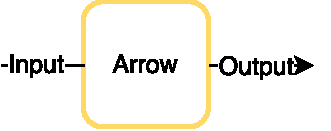
\includegraphics{images/arrow}
\vfill
%	\caption{Schematic depiction of an Arrow.}
%\label{fig:arrow-sch}
}
\parbox[c][17em]{0.49\linewidth}{%
\vfill
\centering
	{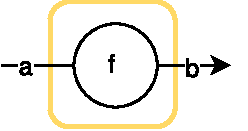
\includegraphics[scale=0.6]{images/arr}}
	{\includegraphics[scale=0.6]{images/compose}}
	{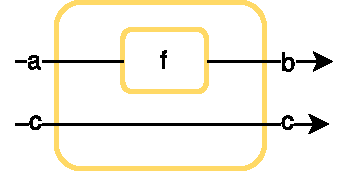
\includegraphics[scale=0.6]{images/first}}
\vfill
%\caption{Schematic depiction of |Arrow| combinators |arr|, |>>>| and |first|.}
%\label{fig:arrows-viz}
}
\caption{Schematic depiction of  an Arrow (left) and its basic
  combinators |arr|, |>>>| and |first| (right).}
\label{fig:arrow-sch}
\label{fig:arrows-viz}
\end{figure}

\subsection{Arrows}
\label{sec:arrows}
Arrows were introduced by \citet{HughesArrows} as a general interface for computation. An Arrow |arr a b| represents  a computation that converts an input |a| to an output |b|. This is defined in the |Arrow| type class shown in Fig.~\ref{fig:ArrowDefinition}.
%
To lift an ordinary function to an Arrow, |arr| is used, analogous to the monadic |return|. Similarly, the composition operator |>>>| is analogous to the monadic composition |>>=| and combines two arrows |arr a b| and |arr b c| by \enquote{wiring} the outputs of the first to the inputs to the second to get a new arrow |arr a c|. Lastly, the |first| operator takes the input Arrow |arr a b| and converts it into an arrow on pairs |arr (a, c) (b, c)| that leaves the second argument untouched. It allows us to to save input across arrows. Figure~\ref{fig:arrows-viz} shows a graphical representation of these basic Arrow combinators.
The most prominent instances of this interface are regular functions |(->)|
and the Kleisli type (Fig.~\ref{fig:ArrowDefinition}), which wraps monadic functions, e.g.  |a -> m b| (with |m| being a Monad).

\begin{figure}[h]
	\centering
	\begin{tabular}{cc}
		% \subcaptionbox
{\label{t1}}{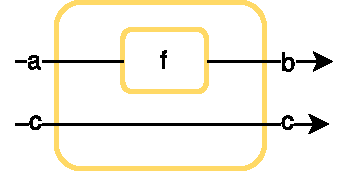
\includegraphics[width = 1.5in]{images/first}} &
		% \subcaptionbox
{\label{fig:secondImg}}{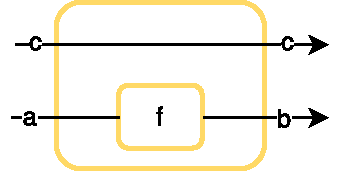
\includegraphics[width = 1.5in]{images/second}} \\
|first| & |second| \\
\midrule
		% \subcaptionbox
{}{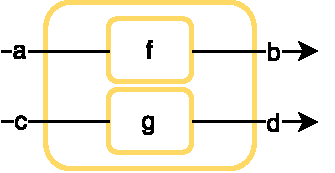
\includegraphics[width = 1.5in]{images/starstarstar}} &
		% \subcaptionbox
{}{\includegraphics[width = 1.5in]{images/andandand}}\\
|(***)|\label{fig:***Img} & |(&&&)| \label{fig:&&&Img} \\
	\end{tabular}
	\caption{Visual depiction of syntactic sugar for Arrows.}
	\label{fig:syntacticSugarArrows}
\end{figure}
Hughes also defined some syntactic sugar (Fig.~\ref{fig:syntacticSugarArrows}): |second|, |***| and |&&&|. 
|second| is the mirrored version of |first| (Appendix~\ref{utilfns}).
|***| combines |first| and |second| to handle two inputs in one arrow, and is defined as follows:
% \begin{figure}[h]
\begin{code}
(***) :: Arrow arr => arr a b -> arr c d -> arr (a, c) (b, d)
f *** g = first f >>> second g
\end{code}
% \caption{The (***) combinator}
% \label{fig:***}
% \end{figure}
The |&&&| combinator, which constructs an Arrow that outputs two different values like |***|, but takes only one input, is:
% \begin{figure}[h]
\begin{code}
(&&&) :: Arrow arr => arr a b -> arr a c -> arr a (b, c)
f &&& g = arr (\a -> (a, a)) >>> (f *** g)
\end{code}
% \caption{The (\&\&\&) combinator}
% \label{fig:&&&}
% \end{figure}
A~first short example given by Hughes on how to use arrows is addition with arrows:
%|add| over arrows, which can be seen in Fig.~\ref{fig:addArrows}.
% \begin{figure}[h]
\begin{code}
add :: Arrow arr => arr a Int -> arr a Int -> arr a Int
add f g = (f &&& g) >>> arr (\(u, v) -> u + v)
\end{code}
% \caption{Add over arrows}
% \label{fig:addArrows}
% \end{figure}
% The benefit of using the |Arrow| typeclass is that any type which is shown to be an arrow can be used in conjunction with this newly created |add| combinator. Even though this example is quite simple, the power of the arrow interface immediately is clear: If a type is an arrow, it can automatically used together with every library that works on arrows. Compared to simple Monads, this enables us to write code that is more extensible, without touching the internals of the specific arrows.
% \\\\
% \textit{Note: In the definitions Hughes gave in his paper, the notation |a b c| for an arrow from |b| to |c| is used. We use the equivalent definition |arr a b| for an arrow from |a| to |b| instead, to make it easier to find the arrow type in type signatures.}
%

The more restrictive interface of Arrows allows for more elaborate composition and transformation combinators---a Monad can be \emph{anything}, an Arrow is a process of doing something, a \emph{computation}. This is exactly one of the key challenges in parallel computing.


%%% Local Variables:
%%% mode: latex
%%% TeX-master: "main"
%%% End:

	\section{Background}
\label{sec:background}
\subsection{Short introduction to parallel Haskells}
There are already several ways to write parallel programs in Haskell. As we will base our parallel arrows on existing parallel Haskells, we will now give a short introduction to the ones we use as backends in this paper.

In its purest form, parallel computation (on functions) can be looked at as the execution of some functions \inlinecode{a -> b} in parallel:

\begin{figure}[h]
%\begin{lstlisting}[frame=htrbl]
\begin{code}
parEvalN :: [a -> b] -> [a] -> [b]
\end{code}
%\end{lstlisting}
\caption{parEvalN's type signature}
\label{fig:parEvalNTypeSig}
\end{figure}
\begin{figure}[h]
	\includegraphics[scale=0.7]{images/parEvalN}
	\caption{Schematic illustration of parEvalN}
	\label{fig:parEvalN}
\end{figure}
\olcomment{make them to real figures? with environment, reference and such?}
Before we go into detail on how we can use this idea of parallelism for parallel Arrows, as a short introduction to parallelism in Haskell we will now implement \inlinecode{parEvalN} with several different parallel Haskells.

\subsubsection{Multicore Haskell}
Multicore Haskell \cite{Marlow2009,Trinder1999} is way to do parallel processing found in standard GHC.\footnote{Multicore Haskell on Hackage is available under \url{https://hackage.haskell.org/package/parallel-3.2.1.0}, compiler support is integrated in the stock GHC.} It ships with parallel evaluation strategies \cite{Trinder1998a,Marlow2010} for several types which can be applied with \inlinecode{using :: a -> Strategy a -> a}. For \inlinecode{parEvalN} this means that we can just apply the list of functions \inlinecode{[a -> b]} to the list of inputs \inlinecode{[a]} by zipping them with the application operator \inlinecode{\$}. We then evaluate this lazy list \inlinecode{[b]} according to a \inlinecode{Strategy [b]} with the \inlinecode{using :: a -> Strategy a -> a} operator. We construct this strategy with \inlinecode{parList :: Strategy a -> Strategy [a]} and \inlinecode{rdeepseq :: NFData a => Strategy a} where the latter is a strategy which evalutes to normal form. To ensure that programs that use \inlinecode{parEvalN} have the correct evaluation order, we annotate the computation with \inlinecode{pseq :: a -> b -> b} which forces the compiler to not reorder multiple \inlinecode{parEvalN} computations. This is particularly necessary in circular communication topologies like in the \inlinecode{torus} or \inlinecode{ring} skeleton that we will see in chapter \ref{sec:topology-skeletons} which resulted in deadlock scenarios when executed without \inlinecode{pseq} during testing for this paper.

\begin{lstlisting}[frame=htrbl]
parEvalN :: (NFData b) => [a -> b] -> [a] -> [b]
parEvalN fs as = let bs = zipWith ($) fs as in
	(bs `using` parList rdeepseq) `pseq` bs
\end{lstlisting}
\begin{figure}[h]
	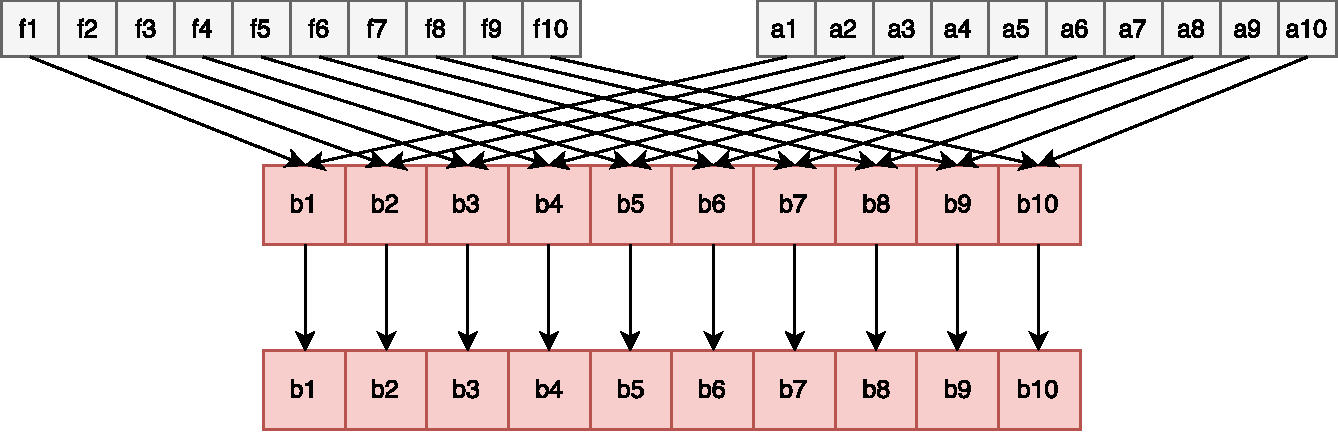
\includegraphics[scale=0.5]{images/parEvalNMulticore}
	\caption{Dataflow of the Multicore Haskell parEvalN version}
\end{figure} %$ %% formatting

\subsubsection{ParMonad}
The \inlinecode{Par} monad\footnote{It can be found in the \texttt{monad-par} package on hackage under \url{https://hackage.haskell.org/package/monad-par-0.3.4.8/}.} introduced by \citet{monad_par_paper_2011}, is a monad designed for composition of parallel programs.


Our parallel evaluation function \inlinecode{parEvalN} can be defined by zipping the list of \inlinecode{[a -> b]} with the list of inputs \inlinecode{[a]} with the application operator \inlinecode{\$} just like with Multicore Haskell. Then, we map over this not yet evaluated lazy list of results \inlinecode{[b]} with \inlinecode{spawnP :: NFData a => a -> Par (IVar a)} to transform them to a list of not yet evaluated forked away computations \inlinecode{[Par (IVar b)]}, which we convert to \inlinecode{Par [IVar b]} with \inlinecode{sequenceA}. We wait for the computations to finish by mapping over the \inlinecode{IVar b}'s inside the \inlinecode{Par} monad with \inlinecode{get}. This results in \inlinecode{Par [b]}. We finally execute this process with \inlinecode{runPar} to finally get \inlinecode{[b]} again.

\textbf{\textcolor{red}{explain problems with laziness here. Problems with torus}}

\begin{lstlisting}[frame=htrbl]
parEvalN :: (NFData b) => [a -> b] -> [a] -> [b]
parEvalN fs as = runPar $ 
	(sequenceA $ map (spawnP) $ zipWith ($) fs as) >>= mapM get
\end{lstlisting}
\begin{figure}[h]
	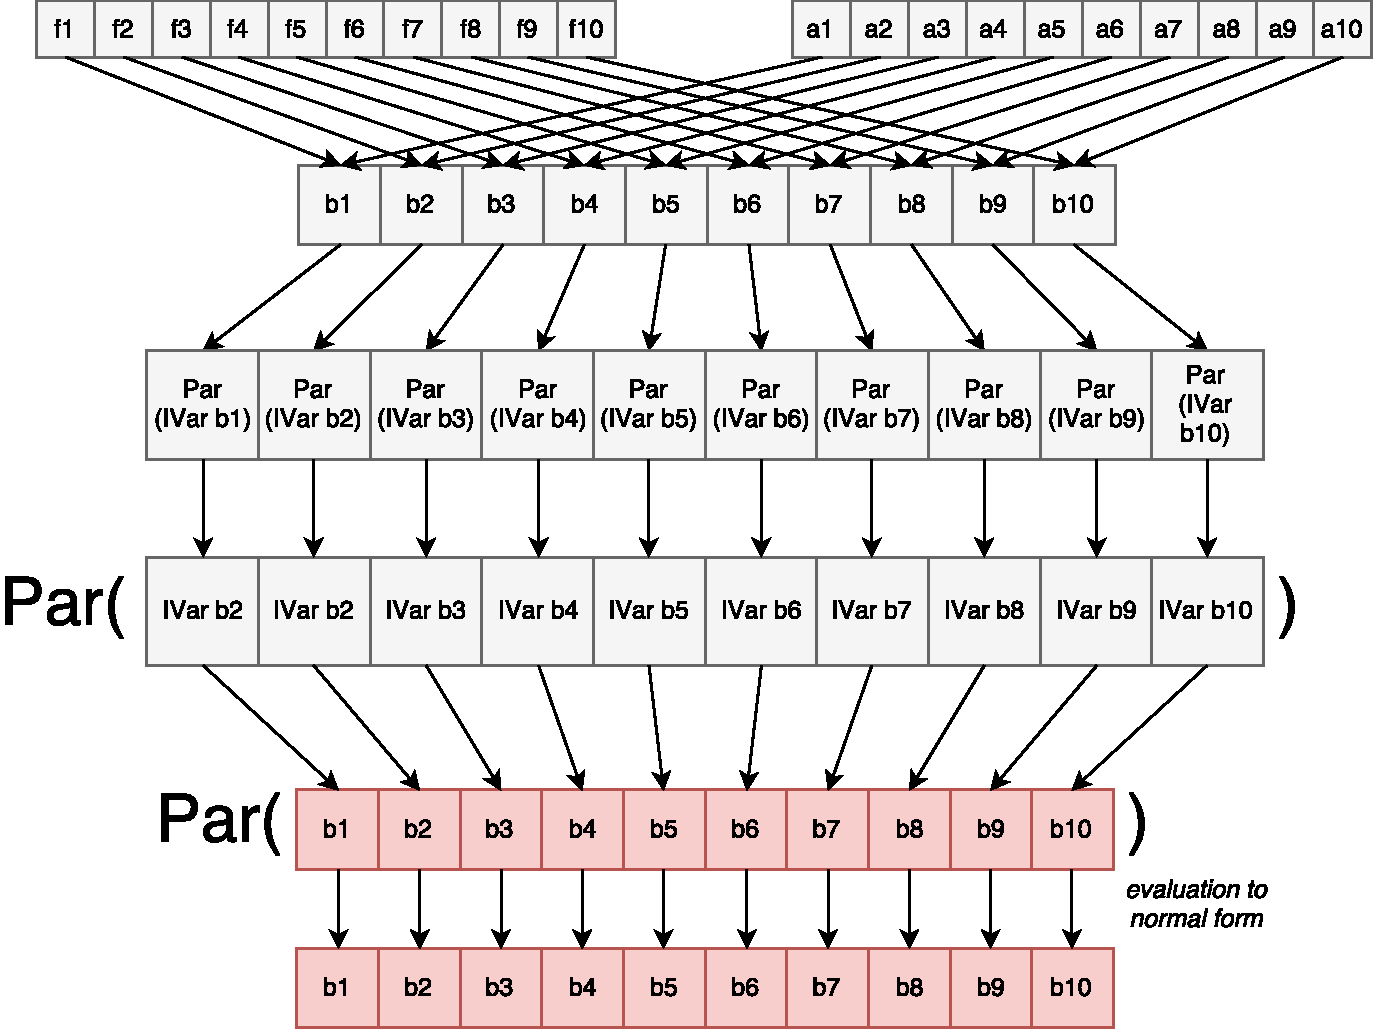
\includegraphics[scale=0.5]{images/parEvalNParMonad}
	\caption{Dataflow of the Par Monad parEvalN version}
\end{figure}

\subsubsection{Eden}
Eden \cite{eden,Loogen2012} is a parallel Haskell for distributed memory and comes with a MPI and a PVM backends.\footnote{See also \url{http://www.mathematik.uni-marburg.de/~eden/} and \url{https://hackage.haskell.org/package/edenmodules-1.2.0.0/}.} This means that it works on clusters as well so it makes sense to have a Eden-based backend for our new parallel Haskell flavour.

Eden was designed to work on clusters, but with a further simple backend it operates on multicores. However, in contrast to many other parallel Haskells, in Eden each process has its own heap. This seems to be a waste of memory, but with distributed programming paradigm and individual GC per process, Eden yields good performance results also on multicores \cite{arcs-dc,aswad2009low}.

While Eden also comes with a monad \inlinecode{PA} for parallel evaluation, it also ships with a completely functional interface that includes
%\\
%\inlinecode{spawnF :: (Trans a, Trans b) => [a -> b] -> [a] -> [b]}.
%\\
a \inlinecode{spawnF} function that
%This 
allows us to define \inlinecode{parEvalN} directly:

\begin{lstlisting}[frame=htrbl]
parEvalN :: (Trans a, Trans b) => [a -> b] -> [a] -> [b]
parEvalN = spawnF 
\end{lstlisting}
\begin{figure}[h]
	\includegraphics[scale=0.5]{images/parEvalNEden}
	\caption{Dataflow of the Eden parEvalN version}
\end{figure}

\paragraph{Eden TraceViewer.}
To comprehend the efficiency and the lack thereof in a parallel program, an inspection of its execution is extremely helpful. While some large-scale solutions exist \cite{Geimer2010}, the parallel Haskell community mainly utilises the tools Threadscope \cite{Wheeler2009} and Eden TraceViewer\footnote{See ..... on hackage for the last available version of Eden TraceViewer. There was an effort to implement the TraceViewer using modern web technologies \cite{traceviewer-web}.} \cite{Berthold2007a}. In the next sections we will present some \emph{traces}, the post-mortem process diagrams of Eden processes and their activity.

In a trace, the $x$ axis shows the time, the $y$ axis enumerates the machines and processes. A~trace shows a running process in green, a blocked process is red. If the process is \enquote{runnable}, \ie it may run, but does not, it is yellow. The typical reason for then is GC. An inactive machine where no processes are started yet, or all are already terminated, is shows as a blue bar. A~comminication from one process to another is represented with a black arrow. A~stream of communications, \eg a transmitted list is shows as a dark shading between sender and receiver processes.

\olcomment{show example trace or refer to a trace in later figures}


%%% Local Variables:
%%% mode: latex
%%% TeX-master: "main"
%%% End:

	%\pagebreak
	\section{Related Work}
\label{sec:related-work}

\paragraph{Parallel Haskells.}
Of course, the three parallel Haskell flavours we use as backends: the GpH \cite{Trinder1996,Trinder1998a} parallel Haskell dialect and its multicore version \cite{Marlow2009}, the |Par| Monad \cite{par-monad,Foltzer:2012:MPC:2398856.2364562}, and Eden \cite{eden,Loogen2012} are related to this work. We use these languages as backends: our DSL can switch from one to other at user's command.

HdpH \cite{Maier:2014:HDS:2775050.2633363,stewart_maier_trinder_2016} is an extension of |Par| Monad to heterogeneous clusters. LVish \cite{Kuper:2014:TPE:2666356.2594312} is a communication-centred extension of |Par| Monad.
%
Further parallel Haskell approaches include pH \cite{ph-book}, research work done on distributed variants of GpH \cite{Trinder1996,Aljabri:2013:DIG:2620678.2620682,Aljabri2015}, and low-level Eden implementation \cite{JostThesis,berthold_loidl_hammond_2016}. Skeleton composition \cite{dieterle_horstmeyer_loogen_berthold_2016}, communication \cite{Dieterle2010}, and generation of process networks \cite{Horstmeyer2013} are recent in-focus research topics in Eden. This also includes the definitions of new skeletons \cite{doi:10.1142/S0129626403001380,Eden:PARCO05,Berthold2009-mr,Berthold2009-fft,dieterle2010skeleton,delaEncina2011,Dieterle2013,janjic2013space}.

More different approaches include data parallelism \cite{Chakravarty2007,Keller:2010:RSP:1932681.1863582}, GPU-based approaches \cite{Mainland:2010:NEC:2088456.1863533,obsidian-phd}, software transactional memory \cite{Harris:2005:CMT:1065944.1065952,Perfumo:2008:LST:1366230.1366241}.
%
The Haskell--GPU bridge Accelerate \cite{Chakravarty:2011:AHA:1926354.1926358,CMCK14,McDonell:2015:TRC:2887747.2804313} deserves a special mention. Accelerate is completely orthogonal to our approach. \citeauthor{marlow2013parallel} authored a recent book in \citeyear{marlow2013parallel} on parallel Haskells.

\paragraph{Algorithmic skeletons.}
Algorithmic skeletons were introduced by \citet{Cole1989}.
Early publications on this topic include \cite{darlington1993parallel,botorog1996efficient,p3l97,Gorlatch1998,Lengauer1997}. \citet{SkeletonBook} consolidated early reports on high-level programming approaches.
The effort is ongoing, including topological skeletons \cite{Eden:PARCO05}, special-purpose skeletons for computer algebra \cite{Berthold2009-fft,lobachev-phd,Lobachev2012,janjic2013space}, iteration skeletons \cite{Dieterle2013}. The idea of \citet{scscp} is to use a parallel Haskell to orchestrate further software systems to run in parallel. \citet{dieterle_horstmeyer_loogen_berthold_2016} compare the composition of skeletons to stable process networks.

\paragraph{Arrows.}
Arrows were introduced by \citet{HughesArrows} as a less restrictive alternative to Monads, basically they are a generalised function arrow~|->|. \citet{Hughes2005} presents a tutorial on Arrows. Some theoretical details on Arrows \cite{jacobs_heunen_hasuo_2009,LINDLEY201197,ATKEY201119} are viable. \citet{Paterson:2001:NNA:507669.507664} introduced a new notation for Arrows. Arrows have applications in information flow research \cite{1648705,LI20101974,Russo:2008:LLI:1411286.1411289}, invertible programming \cite{Alimarine:2005:BAA:1088348.1088357}, and quantum computer simulation \cite{vizzotto_altenkirch_sabry_2006}. But probably most prominent application of Arrows is Arrow-based functional reactive programming, AFRP \cite{Nilsson:2002:FRP:581690.581695,Hudak2003,Czaplicki:2013:AFR:2499370.2462161}.
\citet{Liu:2009:CCA:1631687.1596559} formally define a more special kind of Arrows that capsule the computation more than regular arrows do and thus enable optimizations. Their approach would allow parallel composition, as their special Arrows would not interfere with each other in concurrent execution. In contrast, we capture a whole parallel computation as a single entity: our main instantiation function |parEvalN| makes a single (parallel) Arrow out of list of Arrows. \citet{Huang2007} utilise Arrows for parallelism, but strikingly different from our approach. They use Arrows to orchestrate several tasks in robotics. We, however, propose a general interface for parallel programming, while remaining completely in Haskell.

\paragraph{Other languages.}
Although this work is centered on Haskell implementation of Arrows, it is applicable to any functional programming language where parallel evaluation and Arrows can be defined. Experiments with our approach in Frege language\footnote{GitHub project page at \url{https://github.com/Frege/frege}} (which is basically Haskell on the JVM) were quite successful. A new approach to Haskell on the JVM is the Eta language\footnote{Eta project page at \url{eta-lang.org}}. However, both are beyond the scope of this work.

\citet{achten2004arrows,achten2007arrow} use an Arrow implementation in Clean for better handling of typical GUI tasks. \citet{Dagand:2009:ORD:1481861.1481870} used Arrows in OCaml in the implementation of a distributed system.


%%% Local Variables:
%%% mode: latex
%%% TeX-master: "main"
%%% End:

	%\pagebreak
	%\pagebreak
	\section{Parallel Arrows}
We have seen what Arrows are and how they can be seen as a general interface to computation. In the following section we will discuss how Arrows can also be seen as a general interface not only to computation, but to \textbf{parallel computation} as well. We start by introducing the interface and explaining the reasonings behind it. Then, we discuss some implementations using exisiting parallel Haskells. Finally, we explain why using Arrows for expressing parallelism is beneficial.
\subsection{The ArrowParallel interface}
In its purest form, parallel computation (on functions) can be looked at as the execution of some functions \code{a -> b} in parallel:
\begin{lstlisting}[frame=htrbl]
parEvalN :: [a -> b] -> [a] -> [b]
\end{lstlisting}
Translating this into arrow terms gives us a new operator \code{parEvalN} that lifts a list of arrows \code{[arr a b]} to a parallel arrow \code{arr [a] [b]} (This combinator is similar to our utility function listApp, but does parallel instead of serial evaluation).
\begin{lstlisting}[frame=htrbl]
parEvalN :: (Arrow arr) => [arr a b] -> arr [a] [b]
\end{lstlisting}
With this definition of \code{parEvalN}, parallel execution can be looked at as yet another arrow combinator. But as the implementation may differ depending on the actuall type of the arrow \code{arr} and we want this to be an interface for different backends, we have to introduce the new typeclass \code{ArrowParallel} to host this combinator.
\begin{lstlisting}[frame=htrbl]
class Arrow arr => ArrowParallel arr a b where
	parEvalN :: [arr a b] -> arr [a] [b]
\end{lstlisting}
Sometimes parallel Haskells require additional configuration parameters for information about the execution environment. This is why we also introduce an additional \code{conf} parameter to the function. We also do not want \code{conf} to be of a fixed type, as the configuration parameters can differ for different instances of \code{ArrowParallel}, so we add it to the type signature of the typeclass as well.
\begin{lstlisting}[frame=htrbl]
class Arrow arr => ArrowParallel arr a b conf where
	parEvalN :: conf -> [arr a b] -> arr [a] [b]
\end{lstlisting}
We don't require the conf parameter in every implementation. If it is not needed, we usually want to allow the \code{conf} type parameter to be of any type and don't even evaluate it by blanking it in the type signature of the implemented \code{parEvalN} as we will see in the implementation sections.

\subsection{Multicore Haskell}
The Multicore Haskell implementation of this class is straightforward using listApp from \ref{utilfns} combined with the \code{using} operator from Multicore Haskell.
\begin{lstlisting}[frame=htrbl]
instance (NFData b, ArrowApply arr, ArrowChoice arr) =>
	ArrowParallel arr a b conf where
		parEvalN _ fs = listApp fs >>> arr (flip using $ parList rdeepseq)
\end{lstlisting}
We hardcode the \code{parList rdeepseq} strategy here as in this context it is the only one making sense as we usually want the output list to be fully evaluated to its normal form.

\subsection{ParMonad}
The ParMonad implementation makes use of Haskells laziness and ParMonad's \code{spawnP :: a -> Par (IVar a)} function which forks away the computation of a value and returns an IVar containing the result in the Par monad.
\\\\
We therefore apply each function to its corresponding input value with \code{app} and then fork the computation away with \code{arr spawnP} inside a \code{zipWithArr} call. This yields a list \code{[Par (IVar b)]}, which we then convert into \code{Par [IVar b]} with \code{arr sequenceA}. In order to wait for the computation to finish, we map over the \code{IVar}s inside the ParMonad with \code{arr (>>= mapM get)}. The result of this operation is a \code{Par [b]} from which we can finally remove the monad again by running \code{arr runPar} to get our output of \code{[b]}.
\begin{lstlisting}[frame=htrbl]
instance (NFData b, ArrowApply arr, ArrowChoice arr) =>
	ArrowParallel arr a b conf where
		parEvalN _ fs = 
			(arr $ \as -> (fs, as)) >>>
			zipWithArr (app >>> arr spawnP) >>>
			arr sequenceA >>>
			arr (>>= mapM get) >>>
			arr runPar
\end{lstlisting}

\subsection{Eden}
For the Multicore and ParMonad implementation we could use general implementations that just required the \code{ArrowApply} and \code{ArrowChoice} typeclasses. With Eden this is not the case as we can only spawn a list of functions and we cannot extract simple functions out of arrows. While we could still manage to have only one class in the module by introducing a typeclass like
\begin{lstlisting}[frame=htrbl]
class (Arrow arr) => ArrowUnwrap arr where
	arr a b -> (a -> b)
\end{lstlisting}
we don't do this in this paper, as this seems too hacky. For now, we just implement \code{ArrowParallel} for normal functions
\begin{lstlisting}[frame=htrbl]
instance (Trans a, Trans b) => ArrowParallel (->) a b conf where
parEvalN _ fs as = spawnF fs as
\end{lstlisting}
and the Kleisli type.
\begin{lstlisting}[frame=htrbl]
instance (Monad m, Trans a, Trans b, Trans (m b)) =>
	ArrowParallel (Kleisli m) a b conf where
parEvalN conf fs =
	(arr $ parEvalN conf (map (\(Kleisli f) -> f) fs)) >>>
	(Kleisli $ sequence)
\end{lstlisting}

\subsection{HdpH}

\subsection{Benefits of parallel Arrows}
We have seen that we can wrap parallel Haskells inside of the \code{ArrowParallel} interface, but why do we abstract parallelism this way and what does this approach do better than the other parallel Haskells?
\begin{itemize}
	\item \textbf{Arrow API benefits}:
	With the \code{ArrowParallel} typeclass we do not lose any benefits of using arrows as \code{parEvalN} is just yet another arrow combinator. The resulting arrow can be used in the same way its serial version can be used. This is a big advantage of this approach, especially compared to the monad solutions as all arrow combinators will continue to work instead of requiring special ones for each parallel monad.
	\item \textbf{Abstraction}:
	With the \code{ArrowParallel} typeclass, we abstracted all parallel implementation logic away from the business logic. This gives us the beautiful situation of being able to write our code against the interface the typeclass gives us without being bound to any parallel Haskell. So as an example, during development, we can run the code on the simple Multicore version and afterwards deploy it on a cluster using an Eden built, by just swapping out the actual \code{ArrowParallel} instance.
\end{itemize}

	%\pagebreak
	\section{Basic Skeletons}

With the \code{ArrowParallel} typeclass in place and implemented, we can now implement some basic parallel skeletons.

\subsection{parEvalNLazy}
\begin{center}
	\includegraphics[scale=0.7]{images/parEvalNLazy}
\end{center}
\code{parEvalN} is 100\% strict, which means that it fully evaluates all passed arrows. Sometimes this might not be feasible, as it will not work on infinite lists of functions like e.g. \code{map (arr . (+)) [1..]} or just because we need the arrows evaluated in chunks. \code{parEvalNLazy} fixes this. It works by first chunking the input from \code{[a]} to \code{[[a]]} with the given \code{ChunkSize} in \code{(arr \$ chunksOf chunkSize)}. These chunks are then fed into a list \code{[arr [a] [b]]} of parallel arrows created by feeding chunks of the passed \code{ChunkSize} into the regular parEvalN by using \code{listApp}. The resulting \code{[[b]]} is lastly converted into \code{[b]} with \code{arr concat}.
\begin{lstlisting}[frame=htrbl]
parEvalNLazy :: (ArrowParallel arr a b conf, ArrowChoice arr, ArrowApply arr) =>
	conf -> ChunkSize -> [arr a b] -> (arr [a] [b])
parEvalNLazy conf chunkSize fs =
	arr (chunksOf chunkSize) >>>
	listApp fchunks >>>
	arr concat
	where
		fchunks = map (parEvalN conf) $ chunksOf chunkSize fs
\end{lstlisting}

\subsection{parEval2}
\begin{center}
	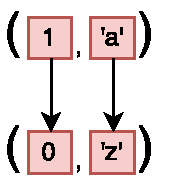
\includegraphics[scale=0.7]{images/parEval2}
\end{center}
We have only talked about the paralellization arrows of the same type until now. But sometimes we want to paralellize heterogenous types as well. For this, we introduce a helper combinator \code{arrMaybe} first, that converts an arrow \code{arr a b} to an arrow \code{arr (Maybe a) (Maybe b)}.
\begin{lstlisting}[frame=htrbl]
arrMaybe :: (ArrowApply arr) => (arr a b) -> arr (Maybe a) (Maybe b)
arrMaybe fn = (arr $ go) >>> app
	where 
		go Nothing = (arr $ \Nothing -> Nothing, Nothing)
		go (Just a) = ((arr $ \(Just x) -> (fn, x)) >>> app >>> arr Just, (Just a))
\end{lstlisting}
With this, we can now easily write \code{parEval2} which combines two arrows \code{arr a b} and \code{arr c d} into a new parallel arrow \code{arr (a, c) (b, d)}. We start by converting both arrows with \code{arrMaybe}, combining them with \code{***} into a new arrow \code{arr (Maybe a, Maybe c) (Maybe b, Maybe d)}. This is then replicated twice and fed into parEvalN to get a \code{arr [(Maybe a, Maybe c)] [(Maybe b, Maybe d)]}. We can then apply this arrow to the input \code{[(Just a, Nothing), (Nothing, Just c)]} and then extract the resulting values with \code{fromJust} and the \code{!!} operator on lists in the last step.
\begin{lstlisting}[frame=htrbl]
parEval2 :: (ArrowParallel arr a b conf,
	ArrowParallel arr (Maybe a, Maybe c) (Maybe b, Maybe d) conf,
	ArrowApply arr) =>
	conf -> arr a b -> arr c d -> (arr (a, c) (b, d))
parEval2 conf f g =
	(arr $ \(a, c) -> (f_g, [(Just a, Nothing), (Nothing, Just c)])) >>>
	app >>>
	(arr $ \comb -> (fromJust (fst (comb !! 0)), fromJust (snd (comb !! 1))))
where
	f_g = parEvalN conf $ replicate 2 $ arrMaybe f *** arrMaybe g
\end{lstlisting}
	%\pagebreak
	\subsubsection{Syntactic Sugar} \label{syntacticSugar}
For basic arrows, we have the \inlinecode{(***)} combinator (Fig.~\ref{fig:***Img},~\ref{fig:***}) which allows us to combine two arrows \inlinecode{arr a b} and \inlinecode{arr c d} into an arrow \inlinecode{arr (a, c) (b, d)} which does both computations at once. This can easily be translated into a parallel version \inlinecode{(|***|)} (Fig.~\ref{fig:|***|}) with the use of \inlinecode{parEval2}, but for this we require a backend which has an implementation that does not require any configuration (hence the \inlinecode{()} as the conf parameter in Fig.~\ref{fig:|***|}).
\begin{figure}[h]
\begin{lstlisting}[frame=htrbl]
(|***|) :: (ArrowChoice arr, ArrowParallel arr (Either a c) (Either b d) ())) =>
	arr a b -> arr c d -> arr (a, c) (b, d)
(|***|) = parEval2 ()
\end{lstlisting}
\caption{Definition of (|***|) - the parallel version of (***)}
\label{fig:|***|}
\end{figure}
% With this we can analogously to the serial \inlinecode{&&&}
We define the parallel \inlinecode{(|\&\&\&|)} (Fig.~\ref{fig:|&&&|}) in a similar manner to its sequential pendant \inlinecode{(\&\&\&)} (Fig.~\ref{fig:&&&Img},~\ref{fig:&&&}).
\begin{figure}[h]
\begin{lstlisting}[frame=htrbl]
(|&&&|) :: (ArrowChoice arr, ArrowParallel arr (Either a a) (Either b c) ()) =>
	arr a b -> arr a c -> arr a (b, c)
(|&&&|) f g = (arr $ \a -> (a, a)) >>> f |***| g
\end{lstlisting} % $ %% formatting
\caption{Definition of (|\&\&\&|) - the parallel version of (\&\&\&)}
\label{fig:|&&&|}
\end{figure}
	%\pagebreak
	\section{Futures} \label{futures}
Consider the parallel arrow combinator in Fig.~\ref{fig:someCombinator}
\begin{figure}[h]
\begin{code}
someCombinator :: (Arrow arr) => [arr a b] -> [arr b c] -> arr [a] [c]
someCombinator fs1 fs2 = parEvalN () fs1 >>> rightRotate >>> parEvalN () fs2
\end{code}
\caption{An example parallel Arrow combinator without Futures.}
\label{fig:someCombinator}
\end{figure}
In a distributed environment, a resulting arrow of this combinator first evaluates all |[arr a b]| in parallel, sends the results back to the master node, rotates the input once and then evaluates the |[arr b c]| in parallel to then gather the input once again on the master node.
Such situations arise, \eg in scientific computations when the data distributed across the nodes needs to be transposed. A concrete example is 2D FFT computation \cite{Gorlatch,Berthold2009-fft}.

While the example in Fig.~\ref{fig:someCombinator} could be rewritten into only one |parEvalN| call by directly wiring the arrows properly together, this example illustrates an important problem: When using a |ArrowParallel| backend that resides on multiple computers, all communication between the nodes is done via the master node, as shown in the Eden trace in Figure~\ref{fig:withoutFutures}. This can become a serious bottleneck %in heavy threaded applications.
for larger amount of data and number of processes \citep[showcases][as, \eg]{Berthold2009-fft}.
\begin{figure}[ht]
	\centering
	\includegraphics[width=0.9\textwidth]{images/withoutFutures}
	\caption[without Futures]{Communication between 4 threads without Futures. All communication goes through the master node. Each bar represents one process. Black lines between processes represent communication. Colors: blue $\hat{=}$ idle, green $\hat{=}$ running, red  $\hat{=}$ blocked, yellow $\hat{=}$ suspended.}
	\label{fig:withoutFutures}
\olcomment{more practical and heavy-weight example! fft (I have the code)?}\\
\mbcomment{Depends... Are the communications easy to read in such an example?}\\
\mbcomment{Keep the description for the different colours, or link to the EdenTV description in \ref{sec:edentv}}
\end{figure}

This motivates for an approach that allows the nodes to communicate directly with each other. Thankfully, Eden, the distributed parallel Haskell we have used in this paper so far, already ships with the concept of |RD| (remote data) that enables this behaviour \cite{AlGo03a,Dieterle2010}.

But as we want code written against our API to be implementation agnostic, we have to wrap this context. We do this with the |Future| typeclass (Fig.~\ref{fig:future}).
\begin{figure}[h]
\begin{code}
class Future fut a | a -> fut where
    put :: (Arrow arr) => arr a (fut a)
    get :: (Arrow arr) => arr (fut a) a
\end{code}
\caption{Definition of the |Future| typeclass.}
\label{fig:future}
\end{figure}
Since |RD| is only a type synonym for communication type that Eden uses internally, we have to use some wrapper classes to fit that definition, though, as seen in Appendix in Fig.~\ref{fig:RDFuture}. This is due to the same reason we had to introduce a wrapper for |Strategy a| in the Multicore Haskell implementation of |ArrowParallel| in Section~\ref{sec:parrows:multicore}.

For our Par Monad and Multicore Haskell backends, we can simply use |MVar|s \cite{jones1996concurrent} (Fig.~\ref{fig:MVarFuture}), because we have shared memory in a single node and don't require Eden's sophisticated communication channels. \fixme{explain MVars}
\begin{figure}[h]
\begin{code}
{-# NOINLINE putUnsafe #-}
putUnsafe :: a -> MVar a
putUnsafe a = unsafePerformIO $ do
    mVar <- newEmptyMVar
    putMVar mVar a
    return mVar

instance (NFData a) => Future MVar a where
    put = arr putUnsafe
    get = arr takeMVar >>> arr unsafePerformIO
\end{code}
\caption{MVar instance of the Future typeclass for the Par Monad and Multicore Haskell backends.}
\label{fig:MVarFuture}
\end{figure} % $

Furthermore, in order for these |Future| types to fit with the |ArrowParallel| instances we gave earlier, we have to give the necessary |NFData| and |Trans| instances, the latter are only needed in Eden. Because |MVar| already ships with a |NFData| instance, we only have to supply two simple instances for our |RemoteData| type:
% \begin{figure}[h]
\begin{code}
instance NFData (RemoteData a) where
    rnf = rnf . rd
instance Trans (RemoteData a)
\end{code}
% \caption{NFData and Trans instances for the RemoteData type. The Trans instance does not have any functions declared as the default implementation suffices here. See \url{https://hackage.haskell.org/package/edenmodules-1.2.0.0/docs/Control-Parallel-Eden.html\#g:5} for more information.}
% \end{figure}
The |Trans| instance does not have any functions declared as the default implementation suffices here.

Going back to our communication example we can use this |Future| concept in order to enable direct communications between the nodes in the following way:
\begin{figure}[h]
\begin{code}
someCombinator :: (Arrow arr) => [arr a b] -> [arr b c] -> arr [a] [c]
someCombinator fs1 fs2 =
	parEvalN () (map (>>> put) fs1) >>>
	rightRotate >>>
	parEvalN () (map (get >>>) fs2)
\end{code}
\caption{The combinator from Fig.~\ref{fig:someCombinator} in parallel.}
\label{fig:someCombinatorParallel}
\end{figure}
In a distributed environment, this gives us a communication scheme with messages going through the master node only if it is needed - similar to what is shown in the trace in Fig.~\ref{fig:withFutures}.\olcomment{Fig.~3 is not really clear. Do Figs 2-3 with a lot of load?}
\begin{figure}[ht]
	\centering
	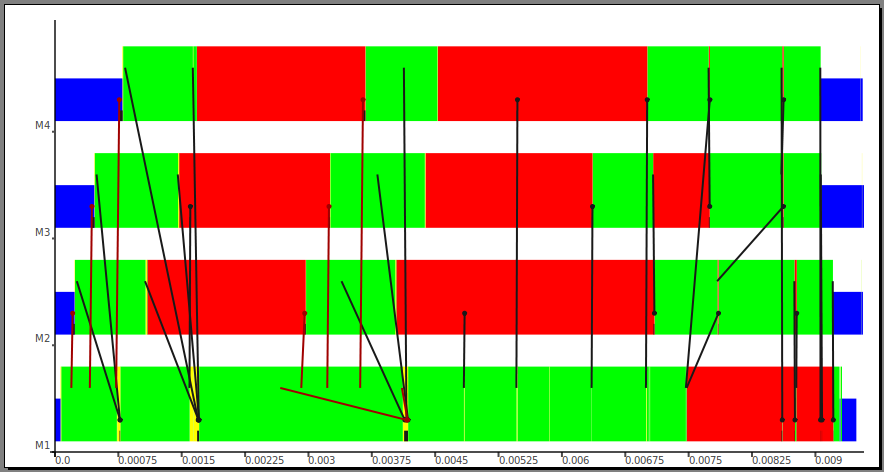
\includegraphics[width=0.9\textwidth]{images/withFutures}
	\caption[with Futures]{Communication between 4 threads with Futures. Other than in Fig.~\ref{fig:withoutFutures}, threads communicate directly (black lines between the bars) instead of always going through the master node (bottom bar).}
	\label{fig:withFutures}
\end{figure}
	%\pagebreak
	\section{Skeletons}
\label{sec:skeletons}
Now we have developed Parallel Arrows far enough to define some useful algorithmic skeletons that abstract typical parallel computations. While there are many possible skeletons to implement, here we only regard in detail some |map|-based and topological skeletons to demonstrate the power of PArrows.
%%% \FloatBarrier
\subsection{|map|-based Skeletons}
\label{sec:map-skeletons}
We start with |map|-based skeletons. The essential differences between the skeletons presented here are in terms of order of evaluation and work distribution but still provide the same output of a standard |map|. 

\paragraph{Parallel |map| and laziness.}
The |parMap| skeleton (Figs.~\ref{fig:parMapImg},~\ref{fig:parMap}) is probably the most common skeleton for parallel programs. We can implement it with |ArrowParallel| by repeating an arrow |arr a b| and then passing it into |parEvalN| to obtain an arrow |arr [a] [b]|.
Just like |parEvalN|, |parMap| traverses all input Arrows as well as the inputs.
Because of this, it has the same restrictions as |parEvalN| as compared to |parEvalNLazy|. So it makes sense to also have a |parMapStream| (Figs.~\ref{fig:parMapStreamImg},~\ref{fig:parMapStream}) which behaves like |parMap|, but uses |parEvalNLazy| instead of |parEvalN|. The code of these two skeletons is quite straightforward, we show it in Appendix \ref{app:omitted} in Figs.\ref{fig:parMap} and \ref{fig:parMapStream}.

\begin{figure}[thb]
%farm
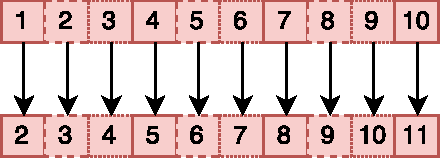
\includegraphics[scale=0.7]{images/farm}
\caption{Schematic depiction of a |farm|, a statically
      load-balanced |parMap|.}
\label{fig:farmImg}

\begin{code}
farm :: (ArrowParallel arr a b conf,
	ArrowParallel arr [a] [b] conf, ArrowChoice arr) =>
	conf -> NumCores -> arr a b -> arr [a] [b]
farm conf numCores f =
	unshuffle numCores >>>
	parEvalN conf (repeat (mapArr f)) >>>
	shuffle
\end{code}
\caption{The definition of |farm|.}
\label{fig:farm}

%farmChunk
\includegraphics[scale=0.7]{images/farmChunk}
\caption{Schematic depiction of |farmChunk|.}
\label{fig:farmChunkImg}
\end{figure}

\paragraph{Statically load-balancing parallel |map|.}
Our |parMap| spawns every single computation in a new thread (at least for the instances of |ArrowParallel| we presented in this paper). This can be quite wasteful and a statically load-balancing |farm| (Figs.~\ref{fig:farmImg},~\ref{fig:farm}) that equally distributes the workload over |numCores| workers seems useful.
The definitions of the helper functions |unshuffle|, |takeEach|, |shuffle| (Fig.~\ref{fig:edenshuffleetc}) originate from an Eden skeleton\footnote{Available on Hackage under \url{https://hackage.haskell.org/package/edenskel-2.1.0.0/docs/src/Control-Parallel-Eden-Map.html}.}.

%\paragraph{Lazy statically load-balancing parallel map}
Since a |farm|  is basically just |parMap| with a different work distribution, it has the same restrictions as |parEvalN| and |parMap|. We can, however, define |farmChunk| (Figs.~\ref{fig:farmChunkImg},~\ref{fig:farmChunk}) which uses |parEvalNLazy| instead of |parEvalN|. It is basically the same definition as for |farm|, but with |parEvalNLazy| instead of |parEvalN|.

%%% Local Variables:
%%% mode: latex
%%% TeX-master: "main"
%%% End:

	%\pagebreak
	%\FloatBarrier
\subsection{Topological skeletons}
\label{sec:topology-skeletons}
Even though many algorithms can be expressed by parallel maps, some problems require more sophisticated skeletons. The Eden library leverages this problem and already comes with more predefined skeletons\footnote{Available on Hackage: \url{https://hackage.haskell.org/package/edenskel-2.1.0.0/docs/Control-Parallel-Eden-Topology.html}.}, among them a |pipe|, a |ring|, and a |torus| implementations \citep{Eden:SkeletonBookChapter02}. These seem like reasonable candidates to be ported to our Arrow-based parallel Haskell. We aim to showcase that we can express more sophisticated skeletons with parallel Arrows as well.

If we used the original definition of |parEvalN|, however, these skeletons would produce an infinite loop with the GpH and |Par| Monad which during runtime would result in the program crash. This materialises with the usage of |loop| of the |ArrowLoop| type class and we think that this is due to difference of how evaluation is done in these backends when compared to Eden. An investigation of why this difference exists is beyond the scope of this work, we only provide a workaround for these types of skeletons as such they probably are not of much importance outside of a distributed memory environment. However our workaround enables users of the DSL to test their code within a shared memory setting.
% even though other skeletons would be better suited to be run with them. --- OL: I don't get this sentence part
The idea of the fix is to provide a |ArrowLoopParallel| type class that has two functions -- |loopParEvalN| and |postLoopParEvalN|, where the first is to be used inside an |loop| construct while the latter will be used right outside of the |loop|. This way we can delegate to the actual |parEvalN| in the spot where the backend supports it.
\begin{code}
class ArrowParallel arr a b conf =>
	ArrowLoopParallel arr a b conf where
    loopParEvalN :: conf -> [arr a b] -> arr [a] [b]
    postLoopParEvalN :: conf -> [arr a b] -> arr [a] [b]
\end{code}
As Eden has no problems with the looping skeletons, we use this instance:
\begin{code}
instance (ArrowChoice arr, ArrowParallel arr a b Conf) =>
	ArrowLoopParallel arr a b Conf where
    loopParEvalN = parEvalN
    postLoopParEvalN _ = evalN
\end{code}
As the backends for the |Par| Monad and GpH have problems with |parEvalN| inside of |loop| their respective instances for |ArrowLoopParallel| look like this:
\begin{code}
instance (ArrowChoice arr, ArrowParallel arr a b (Conf b)) =>
	ArrowLoopParallel arr a b (Conf b) where
    loopParEvalN _ = evalN
    postLoopParEvalN = parEvalN
\end{code}

\subsubsection{Parallel pipe}\label{sec:pipe}

The parallel |pipe| skeleton is semantically equivalent to folding over a list |[arr a a]| of Arrows with |>>>|, but does this in parallel, meaning that the Arrows do not have to reside on the same thread/machine. We implement this skeleton using the |ArrowLoop| type class which gives us the |loop :: arr (a, b) (c, b) -> arr a c| combinator which allows us to express recursive fix-point computations in which output values are fed back as input. For example %this
\begin{code}
loop (arr (\(a, b) -> (b, a:b)))
\end{code}
which is the same as
\begin{code}
loop (arr snd &&& arr (uncurry (:)))
\end{code}
defines an Arrow that takes its input |a| and converts it into an infinite stream |[a]| of it. Using |loop| to our advantage gives us a first draft of a pipe implementation (Fig.~\ref{fig:pipeSimple}) by plugging in the parallel evaluation call |evalN conf fs| inside the second argument of |&&&| and then only picking the first element of the resulting list with |arr last|.

\begin{figure}[t]
\begin{code}
pipeSimple :: (ArrowLoop arr, ArrowLoopParallel arr a a conf) =>
	conf -> [arr a a] -> arr a a
pipeSimple conf fs =
    loop (arr snd &&&
        (arr (uncurry (:) >>> lazy) >>> loopParEvalN conf fs)) >>>
    arr last
\end{code}
\caption{Simple |pipe| skeleton. The use of |lazy| (Fig.~\ref{fig:edenlazyrightrotate}) is essential as without it programs using this definition would never halt. We need to enforce that the evaluation of the input |[a]| terminates before passing it into |evalN|.}
\label{fig:pipeSimple}
\end{figure}

However, using this definition directly will make the master node a potential bottleneck in distributed environments as described in Section~\ref{futures}. Therefore, we introduce a more sophisticated version that internally uses Futures and obtain the final definition of |pipe| in Fig.~\ref{fig:pipe}.

\begin{figure}[t]
\begin{code}
pipe :: (ArrowLoop arr, ArrowLoopParallel arr (fut a) (fut a) conf,
	Future fut a conf) =>
	conf -> [arr a a] -> arr a a
pipe conf fs = unliftFut conf (pipeSimple conf (map (liftFut conf) fs))

liftFut :: (Arrow arr, Future fut a conf, Future fut b conf) =>
	conf -> arr a b -> arr (fut a) (fut b)
liftFut conf f = get conf >>> f >>> put conf

unliftFut :: (Arrow arr, Future fut a conf, Future fut b conf) =>
	conf -> arr (fut a) (fut b) -> arr a b
unliftFut conf f = put conf >>> f >>> get conf
\end{code}
\caption{|pipe| skeleton definition with Futures.}
\label{fig:pipe}
\end{figure}


Sometimes, this |pipe| definition can be a bit inconvenient, especially if we want to pipe Arrows of mixed types together, i.e. |arr a b| and |arr b c|. By wrapping these two Arrows inside a bigger Arrow |arr (([a], [b]), [c]) (([a], [b]), [c])| suitable for |pipe|, we can define |pipe2| as in Fig.~\ref{fig:pipe2}.
\begin{figure}[tb]
\begin{code}
pipe2 :: (ArrowLoop arr, ArrowChoice arr,
    ArrowLoopParallel arr (fut (([a], [b]), [c])) (fut (([a], [b]), [c])) conf,
    Future fut (([a], [b]), [c]) conf) =>
	conf -> arr a b -> arr b c -> arr a c
pipe2 conf f g =
    (arr return &&& arr (const [])) &&& arr (const []) >>>
    pipe conf (replicate 2 (unify f g)) >>>
    arr snd >>>
    arr head
    where
        unify :: (ArrowChoice arr) => 
			arr a b -> arr b c -> arr (([a], [b]), [c]) (([a], [b]), [c])
        unify f' g' =
			(mapArr f' *** mapArr g') *** arr (const []) >>>
			arr (\((b, c), a) -> ((a, b), c))

(parcomp) :: (ArrowLoop arr, ArrowChoice arr,
    ArrowLoopParallel arr (fut (([a], [b]), [c])) (fut (([a], [b]), [c])) (),
    Future fut (([a], [b]), [c]) ()) =>
    arr a b -> arr b c -> arr a c
(parcomp) = pipe2 ()
\end{code}
\caption{Definition of |pipe2| and |(parcomp)|, a parallel |>>>|.}
\label{fig:pipe2}
\end{figure}

Note that extensive use of |pipe2| over |pipe| with a hand-written combination data type will probably result in worse performance because of more communication overhead from the many calls to |parEvalN| inside of |evalN|. Nonetheless, we can define a parallel piping operator |parcomp|, which is semantically equivalent to |>>>| similarly to other parallel syntactic sugar from Appendix~\ref{syntacticSugar}.


%Another version of |>>>| is:
%\begin{code}
%f parcomp g = (f . put) >>> (get . g)
%\end{code}
%It does not launch both Arrows |f| and |g| in parallel, but allows for more smooth data communication between them. Basically, it is a |Future|-lifted \emph{sequential} |>>>|, a way to compose parallel Arrows efficiently.

\subsubsection{Ring skeleton} \label{sec:ring}
\begin{figure}[tb]
	\includegraphics[scale=0.75]{images/ring}
	\caption{|ring| skeleton depiction.}
	\label{fig:ringImg}
\end{figure}
Eden comes with a ring skeleton\footnote{Available on Hackage: \url{https://hackage.haskell.org/package/edenskel-2.1.0.0/docs/Control-Parallel-Eden-Topology.html}} (Fig.~\ref{fig:ringImg}) implementation that allows the computation of a function |[i] -> [o]| with a ring of nodes that communicate with each other. Its input is a node function |i -> r -> (o, r)| in which |r| serves as the intermediary output that gets send to the neighbour of each node. This data is sent over direct communication channels, the so called \enquote{remote data}. We depict it in Appendix, Fig.~\ref{fig:ringEden}.
%\end{code}
%with toRD (to make use of remote data)
%\begin{code}
%\end{code}
%and rightRotate:
%\begin{code}


We can rewrite this functionality easily with the use of |loop| as the definition of the node function, |arr (i, r) (o, r)|, after being transformed into an Arrow, already fits quite neatly into |loop|'s signature: |arr (a, b) (c, b) -> arr a c|. In each iteration we start by rotating the intermediary input from the nodes |[fut r]| with |second (rightRotate >>> lazy)| (Fig.~\ref{fig:edenlazyrightrotate}). Similarly to the |pipe| from Section~\ref{sec:pipe} (Fig.~\ref{fig:pipeSimple}), we have to feed the intermediary input into our |lazy| (Fig.~\ref{fig:edenlazyrightrotate}) Arrow here, or the evaluation would fail to terminate. The reasoning is explained by \citet{Loogen2012} as a demand problem.

Next, we zip the resulting |([i], [fut r])| to |[(i, fut r)]| with |arr (uncurry zip)|. We then feed this into our parallel Arrow |arr [(i, fut r)] [(o, fut r)]| obtained by transforming our input Arrow |f :: arr (i, r) (o, r)| into |arr (i, fut r) (o, fut r)| before |repeat|ing and lifting it with |loopParEvalN|. Finally we unzip the output list |[(o, fut r)]| list into |([o], [fut r])|.

Plugging this Arrow |arr ([i], [fut r]) ([o], fut r)| into the definition of |loop| from earlier gives us |arr [i] [o]|, our ring Arrow (Fig.~\ref{fig:ringFinal}). To make sure this algorithm has speedup on shared-memory machines as well, we pass the result of this Arrow to |postLoopParEvalN conf (repeat (arr id))|.
This combinator can, for example, be used to calculate the shortest paths in a graph using Warshall's algorithm.
%Further details on this can be found in \cite{eden_cefp}.

\begin{figure}[tb]
\begin{code}
ring :: (Future fut r conf,
    ArrowLoop arr,
    ArrowLoopParallel arr (i, fut r) (o, fut r) conf,
    ArrowLoopParallel arr o o conf) =>
    conf -> arr (i, r) (o, r) -> arr [i] [o]
ring conf f =
    loop (second (rightRotate >>> lazy) >>>
        arr (uncurry zip) >>>
        loopParEvalN conf (repeat (second (get conf) >>> f >>> second (put conf))) >>>
        arr unzip) >>>
    postLoopParEvalN conf (repeat (arr id))
\end{code}
\caption{|ring| skeleton definition.}
\label{fig:ringFinal}
\end{figure}

\subsubsection{Torus skeleton}\label{sec:torus}
\begin{figure}
	\includegraphics[scale=0.75]{images/torus}
	\caption{|torus| skeleton depiction.}
	\label{fig:ringTorusImg}
\end{figure}
If we take the concept of a |ring| from Section~\ref{sec:ring} one dimension further, we obtain a |torus| skeleton (Fig.~\ref{fig:ringTorusImg},~\ref{fig:torus}). Every node sends and receives data from horizontal and vertical neighbours in each communication round.
With our Parallel Arrows we re-implement the |torus| combinator\footnote{Available on Hackage: \url{https://hackage.haskell.org/package/edenskel-2.1.0.0/docs/Control-Parallel-Eden-Topology.html}.} from Eden---yet again with the help of the |ArrowLoop| type class.

Similar to the |ring|, we start by rotating the input (Fig.~\ref{fig:edenlazyrightrotate}), but this time not only in one direction, but in two. This means that the intermediary input from the neighbour nodes has to be stored in a tuple |([[fut a]], [[fut b]])| in the second argument (loop only allows for two arguments) of our looped Arrow |arr ([[c]], ([[fut a]], [[fut b]])) ([[d]], ([[fut a]], [[fut b]]))| and our rotation Arrow becomes 
\begin{code}
second ((mapArr rightRotate >>> lazy) *** (arr rightRotate >>> lazy))
\end{code}
instead of the singular rotation in the ring as we rotate |[[fut a]]| horizontally and |[[fut b]]| vertically. Then, we zip the inputs for the input Arrow with 
\begin{code}
arr (uncurry3 zipWith3 lazyzip3)
\end{code}
from |([[c]], ([[fut a]], [[fut b]]))| to |[[(c, fut a, fut b)]]|, which we then evaluate in parallel.

This, however, is more complicated than in the ring case as we have one more dimension of inputs that needs to be transformed. We first have to |shuffle| all the inputs to then pass them into |loopParEvalN conf (repeat (ptorus conf f))| to get an output of |[(d, fut a, fut b)]|. We then unshuffle this list back to its original ordering by feeding it into |arr (uncurry unshuffle)| which takes the input length we saved one step earlier as additional input to get a result matrix |[[[(d, fut a, fut b)]]|. Finally, we unpack this matrix  with |arr (map unzip3) >>> arr unzip3 >>> threetotwo| to get |([[d]], ([[fut a]], [[fut b]]))|.

This internal looping computation is once again fed into |loop| and we also compose a final |postLoopParEvalN conf (repeat (arr id))| for the same reasons as explained for the |ring| skeleton. 

\begin{figure}[tb]
\begin{code}
torus :: (Future fut a conf, Future fut b conf,
      ArrowLoop arr, ArrowChoice arr,
      ArrowLoopParallel arr (c, fut a, fut b) (d, fut a, fut b) conf,
      ArrowLoopParallel arr [d] [d] conf) =>
      conf -> arr (c, a, b) (d, a, b) -> arr [[c]] [[d]]
torus conf f =
    loop (second ((mapArr rightRotate >>> lazy) *** (arr rightRotate >>> lazy)) >>>
        arr (uncurry3 (zipWith3 lazyzip3)) >>>
        arr length &&& (shuffle >>> loopParEvalN conf (repeat (ptorus conf f))) >>>
        arr (uncurry unshuffle) >>>
        arr (map unzip3) >>> arr unzip3 >>> threetotwo) >>>
    postLoopParEvalN conf (repeat (arr id))

ptorus :: (Arrow arr, Future fut a conf, Future fut b conf) =>
          conf ->
          arr (c, a, b) (d, a, b) ->
          arr (c, fut a, fut b) (d, fut a, fut b)
ptorus conf f =
	arr (\ ~(c, a, b) -> (c, get conf a, get conf b)) >>>
	f >>>
	arr (\ ~(d, a, b) -> (d, put conf a, put conf b))
\end{code} % $
\caption{|torus| skeleton definition. |lazyzip3|, |uncurry3| and |threetotwo| definitions are in Fig.~\ref{fig:lazyzip3etc}}.
\label{fig:torus}
\end{figure}
As an example of using this skeleton, \citet{Eden:SkeletonBookChapter02} showed the matrix multiplication using the Gentleman algorithm (\citeyear{Gentleman1978}). An adapted version can be found in Fig.~\ref{fig:torusMatMult}.
\begin{figure}[tb]
\begin{code}
type Matrix = [[Int]]

prMM_torus :: Int -> Int -> Matrix -> Matrix -> Matrix
prMM_torus numCores problemSizeVal m1 m2 =
	combine $ torus () (mult torusSize) $ zipWith (zipWith (,)) (split m1) (split m2)
    	where   torusSize = (floor . sqrt) $ fromIntegral numCores
            	combine = concat . (map (foldr (zipWith (++)) (repeat [])))
            	split = splitMatrix (problemSizeVal `div` torusSize)

-- Function performed by each worker
mult :: Int -> ((Matrix,Matrix),[Matrix],[Matrix]) -> (Matrix,[Matrix],[Matrix])
mult size ((sm1,sm2),sm1s,sm2s) = (result,toRight,toBottom)
    where toRight = take (size-1) (sm1:sm1s)
          toBottom = take (size-1) (sm2':sm2s)
          sm2' = transpose sm2
          sms = zipWith prMMTr (sm1:sm1s) (sm2':sm2s)
          result = foldl1' matAdd sms
\end{code} %$
\caption{Adapted matrix multiplication in Eden using a the |torus| skeleton. |prMM_torus| is the parallel matrix multiplication. |mult| is the function performed by each worker. |prMMTr| calculates $AB^T$ and is used for the (sequential) calculation in the chunks. |splitMatrix| splits the Matrix into chunks. |matAdd| calculates $A + B$. Omitted definitions can be found in \ref{fig:torus_example_rest}. }
\label{fig:torusMatMult}
\end{figure}
If we compare the trace from a call using our Arrow definition of the torus (Fig.~\ref{fig:torus_parrows_trace}) with the Eden version (Fig.~\ref{fig:torus_eden_trace}) we can see that the behaviour of the Arrow version and execution times are comparable. We discuss further benchmarks on larger clusters and in a more detail in the next section.
\begin{figure}[tb]
\olcomment{more nodes!!!}
	\centering
	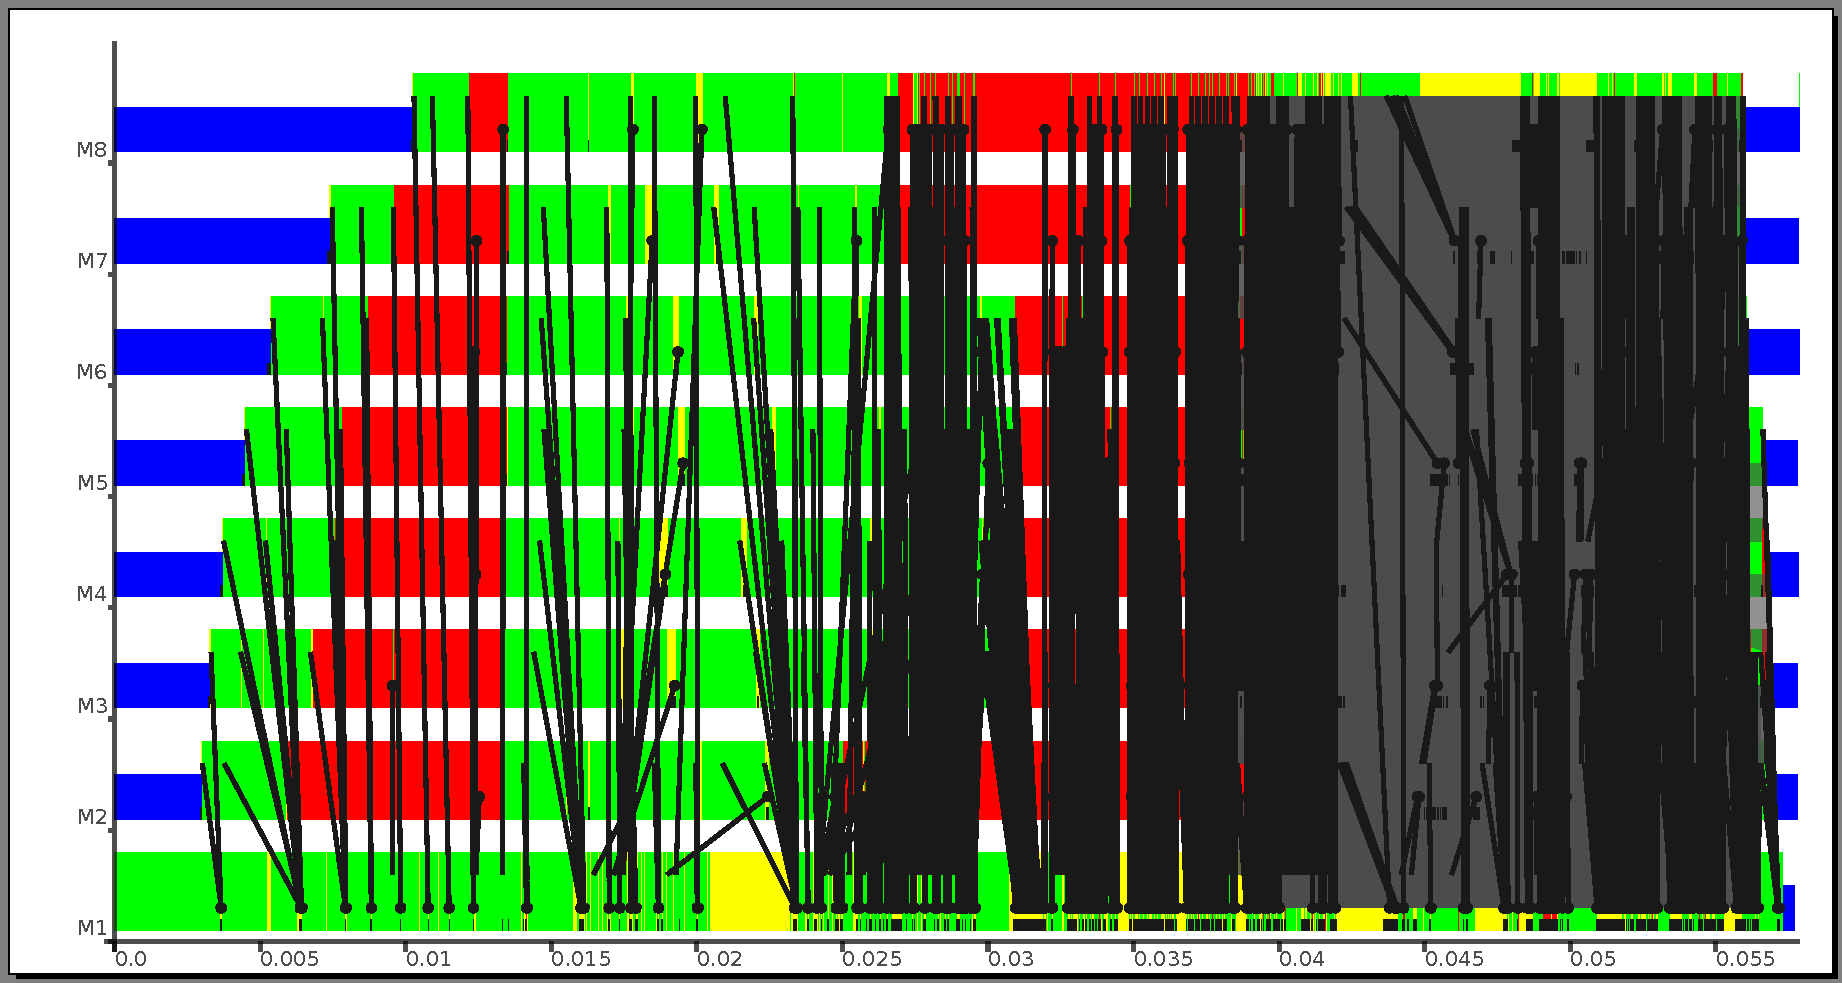
\includegraphics[width=0.9\textwidth]{images/torus_matrix_parrows_scale}
	\caption[Matrix multiplication with |torus| (PArrows)]{Matrix multiplication with |torus| (PArrows).}
	\label{fig:torus_parrows_trace}
\end{figure}

\begin{figure}[tb]
	\centering
	\includegraphics[width=0.9\textwidth]{images/torus_matrix_eden_scale}
	\caption[Matrix multiplication with |torus| (Eden)]{Matrix multiplication with |torus| (Eden).}
	\label{fig:torus_eden_trace}
\end{figure}

%\FloatBarrier

%%% Local Variables:
%%% mode: latex
%%% TeX-master: "main"
%%% End:

	%\pagebreak
	\section{Performance results}
\label{sec:benchmarks}

\newcommand{\rmtest}{Rabin--Miller test\xspace}
\newcommand{\sudokutest}{Sudoku\xspace}
\newcommand{\jacobitest}{Jacobi sum test\xspace}
\newcommand{\torustest}{Gentleman\xspace}
\newlength{\plotwidthSMP}
\setlength{\plotwidthSMP}{0.39\textwidth}
\newlength{\plotwidthDist}
\setlength{\plotwidthDist}{0.6\textwidth}


\newcommand{\performanceplot}[7]{
\begin{tikzpicture}
\begin{axis}[title={#1},
title style={align=center},
scale only axis, width=#7,
xlabel=Threads,
%xtick=data,
xtick distance=#4,
ylabel=Time (s),
ylabel near ticks,
minor tick num=2,
grid=major,
legend entries={#2},
legend style={at={(0.99,0.99)},anchor=north east},
max space between ticks=50pt,
grid style={line width=.1pt, draw=gray!10},
major grid style={line width=.2pt,draw=gray!50},
xmin=-1,
xmax=#6]
#5
\end{axis}
\end{tikzpicture}
}

\newcommand{\performancediffplot}[8]{
\begin{tikzpicture}
\begin{axis}[title={#1},
title style={align=center},
scale only axis, width=#8,
xlabel=Threads,
%xtick=data,
ytick distance=#6,
xtick distance=#4,
minor tick num=9,
ylabel=Absolute time difference (s),
ylabel near ticks,
grid=both,
legend entries={#2},
legend style={at={(0.99,0.99)},anchor=north east},
max space between ticks=50pt,
grid style={line width=.1pt, draw=gray!10},
major grid style={line width=.2pt,draw=gray!50},
xmin=-1,
xmax=#7]
#5
\end{axis}
\end{tikzpicture}
}

\newcommand{\speedupplot}[7]{
\begin{tikzpicture}
\begin{axis}[title={#1},
title style={align=center},
scale only axis, width=#7,
xlabel=Threads,
%xtick=data,
%ytick=data,
xtick distance=#4,
ytick distance=#4,
ylabel=Speedup,
ylabel near ticks,
grid=major,
legend entries={linear, #2},
legend style={at={(0.01,0.99)},anchor=north west},
max space between ticks=50pt,
grid style={line width=.1pt, draw=gray!10},
major grid style={line width=.2pt,draw=gray!50},
ymin=-1,
xmin=-1,
ymax=#6,
xmax=#6]
\addplot [domain=0:#3, no markers,dotted,thick]{x};
#5
\end{axis}
\end{tikzpicture}
}

\newcommand{\speedupdiffplot}[7]{
\begin{tikzpicture}
\begin{axis}[title={#1},
title style={align=center},
scale only axis, width=#7,
xlabel=Threads,
%xtick=data,
xtick distance=#4,
ytick distance=0.5,
ylabel=Absolute speedup difference,
ylabel near ticks,
grid=major,
legend entries={#2},
legend style={at={(0.99,0.99)},anchor=north east},
max space between ticks=50pt,
grid style={line width=.1pt, draw=gray!10},
major grid style={line width=.2pt,draw=gray!50},
xmin=-1,
xmax=#6]
#5
\end{axis}
\end{tikzpicture}
}

\subsection{Hardware}

We have tested our parallel DSL and algorithmic skeletons implemented
in it. Benchmarks were conducted both in a shared and in a distributed
memory setting. All benchmarks were done on the ``Glasgow grid'', consisting of
16 machines with 2 Intel\SymbReg~Xeon\SymbReg~E5-2640 v2 and 64 GB of DDR3 RAM each. Each processor has 8 cores and 16 (hyper-threaded) threads with a base frequency of 2 GHz and a turbo frequency of 2.50 GHz. This results in a total of 256 cores and 512 threads for the whole cluster. The operating system was Ubuntu 14.04 LTS with Kernel 3.19.0-33. Non-surprisingly, we found that hyper-threaded 32 cores do not behave in the same manner as real 16 cores (numbers here for a single machine). We disregarded the hyper-threading ability in most of the
cases.

We used a single node with 16 real cores as a shared memory testbed
and the whole grid with 256 real cores as a device to test our
distributed memory software.

\subsection{Test programs}

We used multiple tests that originated from different
sources. Most of them are parallel mathematical computations, initially
implemented in Eden. Table~\ref{tab:benches} summarises.

\begin{table}
\caption{The benchmarks we use in this paper.}
\label{tab:benches}
\centering
%% something was wrong with separators in table
\renewcommand{\tabcolsep}{0.5em}
\begin{tabular}{lccll}
\toprule
Name & Area & Type & Origin & Citation \\
\midrule
\rmtest & Mathematics & |parMap+reduce| & Eden & \citet{Lobachev2012}\\
\jacobitest & Mathematics & |workpool+reduce| & Eden & \citet{Lobachev2012}\\
\torustest & Mathematics & |torus| & Eden & \citet{Eden:SkeletonBookChapter02}\\
\sudokutest & Puzzle & |parMap| & |Par| Monad & \citet{par-monad} 
\tablefootnote{actual code from: http://community.haskell.org/~simonmar/par-tutorial.pdf and https://github.com/simonmar/parconc-examples}\\
\bottomrule
\end{tabular}
\end{table}

\rmtest is a probabilistic primality test that iterates multiple (32--256 here)
``subtests''. Should a subtest fail, the input is definitely not a
prime. If all $n$ subtest pass, the input is composite with the
probability of $1/4^{n}$. 

Jacobi sum test or APRCL is also a primality test, that however,
guarantees the correctness of the result. It is probabilistic in the
sense that its run time is not certain. Unlike \rmtest, the subtests
of Jacobi sum test have very different durations. \citet{lobachev-phd}
discusses some optimisations of parallel APRCL. Generic parallel
implementations of \rmtest and APRCL were presented in \citet{Lobachev2012}.

``Gentleman'' is a standard Eden test program, developed
for their |torus| skeleton. It implements a parallel matrix
multiplication \citep{Gentleman1978}. We ported an Eden based version \citep{Eden:SkeletonBookChapter02} to PArrows.

A~parallel Sudoku solver was used by \citet{par-monad} to compare |Par| Monad
to GpH Haskell. We ported it to PArrows.



\subsection{What parallel Haskells run where}

The \ensuremath{\Conid{Par}} monad and GpH Haskell -- in its multicore version (\cite{Marlow2009}) --  can be executed on a shared
memory machines only. Although GpH is available on distributed memory
clusters, and newer distributed memory Haskells such as HdpH exist,
current support of distributed memory in PArrows is limited to
Eden. We used the MPI backend of Eden in a distributed memory
setting. However, for shared memory Eden features a ``CP'' backend
that merely copies the memory blocks between distributed heaps. In
this mode, Eden still operates in the ``nothing shared'' setting, but
is adapted better to multicore machines. We label this version of Eden
in the plots as ``Eden~CP''.



\subsection{Effect of hyper-threading}

The PArrows version of \rmtest on a single node of the Glasgow grid
showed almost linear speedup (Fig.~\ref{fig:bench-rm-sm}). The speedup
of 64-task PArrows/Eden at 16 real cores version was 13.65, the
efficiency was 85.3\%. However, if we increase the number of
requested cores to be 32 -- \ie if we use hyper-threading on 16 real
cores -- the speedup does not increase that well. It is merely 15.99
for 32 tasks with PArrows/Eden. It is worse for other backends.  As
for 64 tasks, we obtain the speedup of 16.12 with PArrows/Eden at 32
hyper-threaded cores and only 13.55 with PArrows/GpH. Efficiency is 50.4\% and 42.3\%, respectively. The Eden
version used here was Eden~CP, the \enquote{share nothing} SMP build.

In the distributed memory setting the same effect ensues. We obtain
plummeting speedup of 124.31 at 512 hyper-threaded cores, whereas it was
213.172 for 256 real cores. Apparently, hyper-threading in the Glasgow
grid fails to execute two parallel Haskell processes with full-fledged
parallelism. For this reason, we did not regard hyper-threaded cores in
our speedup plots in Figs.~\ref{fig:bench-rm-sm}--\ref{fig:sudokuSMBenchmark}.


% rm 11213 32 32-sm speedup eden: 15.993037587283924
% -"- multi: 15.09948017762912
% -"- par: 14.909092857846693

% -"- 64 32-sm speedup eden: 16.118040224478424
% -"- multi: 13.545304115702333
% -"- par: 15.155709987503396

\subsection{Benchmark results}

The difference between, say, PArrows with |Par| Monad backend and a
genuine |Par|
Monad benchmark is very small. To give an example, it is ~0.4\seconds in favour of PArrows for 16 cores (10.8\seconds vs. 11.2\seconds) and ~-0.8\seconds in favour of the |Par| monad for 8 cores (16.1\seconds vs. 16.9\seconds) for
the Sudoku benchmark in the shared memory setting. It is almost invisible in speedup and
(non shown) run time plots. We thus show only the results for the
PArrows-enabled versions.

To show that PArrows induce very small overhead in a distributed context as well, we compare the original Eden
versions of the benchmark to its PArrows-enabled counterpart in the \rmtest, \torustest and \jacobitest benchmarks. We plot execution time differences between measurements for
PArrows and the corresponding backend in a separate plot
(Figs.~\ref{fig:bench-rm-dist}--\ref{fig:torusBenchmark}). As an example, the differences range in
about 0.5\seconds for the execution time of 46\seconds on 256 cores
for distributed \rmtest with PArrows and Eden. For these comparisons, the plots show absolute
time differences that are not relative \wrt the total execution time.
Furthermore, the error bars ends were computed from point-wise maximum of both standard
deviations from both measurements for PArrows and non-PArrows
versions. These are the values provided by the |bench| package that we
used for bench-marking. We call a difference between two versions
significant when the border of the error bar of absolute time
difference is above or below zero. In other words: the time
difference is significant if it is above measurement error.

\subsubsection{\rmtest}\label{sec:rmtest}

\newcommand{\performanceSkelRMSM}[2]{
\performanceplot{Parallel run time of \rmtest \enquote{#2}}{Eden CP, GpH, |Par| Monad}{16}{4}{
\addplot+ [very thick] table [scatter, x="nCores", y="time", col sep=comma, mark=none,
smooth]{benchmarks/sm-rm/bench-sm-rm.bench.skelrm-parr-eden-cp-#1-#2.csv};
\addplot+ [very thick] table [scatter, x="nCores", y="time", col sep=comma, mark=none,
smooth]{benchmarks/sm-rm/bench-sm-rm.bench.skelrm-parr-mult-#1-#2.csv};
\addplot+ [very thick] table [scatter, x="nCores", y="time", col sep=comma, mark=none,
smooth]{benchmarks/sm-rm/bench-sm-rm.bench.skelrm-parr-par-#1-#2.csv};
}{17}{\plotwidthSMP}
}

\newcommand{\speedupSkelRMSM}[2]{
\speedupplot{Speedup of \rmtest \enquote{#2}}{Eden CP, GpH, |Par| Monad}{16}{4}{
\addplot+ [very thick] table [scatter, x="nCores", y="speedup", col sep=comma, mark=none,
smooth]{benchmarks/sm-rm/bench-sm-rm.bench.skelrm-parr-eden-cp-#1-#2.csv};
\addplot+ [very thick] table [scatter, x="nCores", y="speedup", col sep=comma, mark=none,
smooth]{benchmarks/sm-rm/bench-sm-rm.bench.skelrm-parr-mult-#1-#2.csv};
\addplot+ [very thick] table [scatter, x="nCores", y="speedup", col sep=comma, mark=none,
smooth]{benchmarks/sm-rm/bench-sm-rm.bench.skelrm-parr-par-#1-#2.csv};
}{17}{\plotwidthSMP}
}

\newcommand{\speedupSkelRMDist}[4]{
\speedupplot{Speedup of \rmtest \enquote{#1 #2}}{PArrows}{256}{#3}{
% \addplot [mark=*,very thick] table [scatter, x="nCores", y="speedup", col sep=comma, mark=none,
% smooth]{benchmarks/distributed-rm/bench-distributed.bench.skelrm-parrows-11213-#2.csv};
\addplot [mark=*,very thick,blue] table [scatter, x="nCores", y="speedup", col sep=comma, mark=none,
smooth]{benchmarks/distributed-rm/bench-distributed.bench.skelrm-parrows-#1-#2.csv};
% \addplot table [scatter, x="nCores", y="speedup", col sep=comma, mark=none,
% smooth]{benchmarks/distributed-rm/bench-distributed.bench.skelrm-eden-#1-#2.csv};
}{#4}{\plotwidthDist}
}

\newcommand{\performanceSkelRMDistDiff}[5]{
\performancediffplot{Run time differences\\for \rmtest \enquote{#1 #2}}{(Eden $-$ PArrows)}{256}{#3}{
\addplot+[mark=*,very thick,error bars/.cd,
    y dir=both,y explicit] table [x="nCores", y="time", y error="max stddev", col sep=comma, mark=dots,
smooth]{benchmarks/distributed-rm/#1-#2-diff.csv};
}{#4}{#5}{\plotwidthDist}
}

\begin{figure}
%\centering
%\performanceSkelRMSM{11213}{64}\hfill%
{\speedupSkelRMSM{11213}{32}}\hfill%
{\speedupSkelRMSM{11213}{64}}
\caption{Relative speedup of \rmtest on a multicore machine. We used the same PArrows-based implementation with
  different backends on the same hardware. Measurements were performed on a single node of the Glasgow
  grid; it has 16 real cores. Input was $2^{11213}-1$, we used 32 (left) or 64 (right)
  tasks. The
  closer to linear speedup the better.}
\label{fig:bench-rm-sm}
\end{figure}

\begin{figure}
\centering
%\performanceSkelRMDist{44497}{256}{32,64,128,256,512}{544}
%
{\speedupSkelRMDist{44497}{256}{32}{272}\label{subfig:rm-dist-a}}%
%\hfill%
{\performanceSkelRMDistDiff{44497}{256}{32}{0.5}{272}\label{subfig:rm-dist-b}}
\caption{Parallel performance of \rmtest on the Glasgow grid
  consisting of 256 cores. Input was $2^{44497}-1$, we used 256
  tasks. The top plot shows absolute speedup in a distributed memory setting. The
  closer to linear speedup the better. Time
  (and hence speedup) measurements for PArrows with Eden backend and
  Eden almost coincide. Hence, bottom plot shows
absolute time differences for this benchmark. The
higher the value, the better for PArrows\olcomment{CHECKME}.}
\label{fig:bench-rm-dist}
\end{figure}

\olcomment{THE ACTUAL TEXT IS MISSING. What do we see in the plots?
  Why is it good?}
The multicore version of our parallel \rmtest benchmark is depicted in
Figure~\ref{fig:bench-rm-sm}. We executed the test with 32 and 64
tasks. The plot shows the PArrows-enabled versions with corresponding backends.
The performance of PArrows/Eden~CP in shared memory is slightly better than
for SMP variants such as PArrows/GpH and PArrows/|Par|
Monad but most of the time the performance is still comparable with the GpH backend performing slightly worse than the other two in terms of speedup.

Comparing the PArrows version of the \rmtest with the original from Eden with the MPI backend in a distributed memory setting, we see an almost linear speedup of
\rmtest with 256 tasks and input $2^{44497}-1$ in both versions. The sequential run time
was computed as the mean of three consecutive executions on a single
core---the single run took two hours 43 minutes. The difference between
PArrows/Eden and Eden almost always lies inside the error bar of
the measurement.

%As the PArrows version uses Eden in the backend, these numbers suggest that there is no real performance difference between using PArrows or Eden for this task as they trade blows in this benchmark. Additionally, PArrows with an Eden-based backend performing better than what it is based upon suggests that any difference in runtime between the two is more of an anomaly than a real difference.

\subsubsection{\jacobitest}

Continuing, the results of the \jacobitest (MPI only) in Fig.~\ref{fig:bench-jacobi-dist} are as follows:
The program does not seem to scale well beyond 16-32 tasks with input $2^{3217}-1$. Because of this, we also ran tests with input $2^{4253}-1$, but only for the 128 and 256 cores because of the long running time. For demonstration purposes in Fig.~\ref{fig:bench-jacobi-dist}, we chose a simulated speedup of 22 for 128 cores. For 256 cores, this results in a superlinear speedup of \~122.63, which suggests an IO limitation for this big input that is somewhat mitigated by adding more cores.

We once again compare the Eden version with the PArrrows version in Fig.~\ref{fig:bench-jacobi-dist}. We see similar behaviour to the MPI version of the \rmtest: The difference once again almost always remains within the bounds of the error bar of the measurement.

Not pictured are the slightly bigger differences between Eden and PArrows for the larger input of $2^{4253}-1$: For 128 and 256 cores the differences are -1005.18\seconds and -94.33\seconds in favour of Eden. This maximum of 12.27\% slower PArrows runtime, however, was still in the (quite big) error bar of our measurements.

\newcommand{\speedupJacobiDist}[5]{
\speedupplot{Speedup of \jacobitest \enquote{#2} vs simulated \enquote{#5}}{PArrows #2, simulated PArrows #5}{256}{#3}{
% \addplot [mark=*,very thick] table [scatter, x="nCores", y="speedup", col sep=comma, mark=none,
% smooth]{benchmarks/distributed-rm/bench-distributed.bench.skelrm-parrows-11213-#2.csv};
\addplot [mark=*,very thick,blue] table [scatter, x="nCores", y="speedup", col sep=comma, mark=none,
smooth]{benchmarks/distributed-jacobi/bench-jacobi.bench.jacobi-parr-#1-#2.csv};
\addplot [mark=x,very thick,red] table [scatter, x="nCores", y="speedup", col sep=comma, mark=none,
smooth]{benchmarks/distributed-jacobi/bench-jacobi.bench.jacobi-parr-#1-#5.csv};
% \addplot table [scatter, x="nCores", y="speedup", col sep=comma, mark=none,
% smooth]{benchmarks/distributed-rm/bench-distributed.bench.skelrm-eden-#1-#2.csv};
}{#4}{\plotwidthDist}
}

\newcommand{\performanceJacobiDistDiff}[5]{
\performancediffplot{Run time differences\\for \jacobitest \enquote{#2}}{(Eden $-$ PArrows) #2}{256}{#3}{
\addplot+[mark=*,very thick,error bars/.cd,
    y dir=both,y explicit] table [x="nCores", y="time", y error="max stddev", col sep=comma, mark=dots,
smooth]{benchmarks/distributed-jacobi/#1-#2-diff.csv};
}{#4}{#5}{\plotwidthDist}
}

\begin{figure}
\centering
%\performanceSkelRMDist{44497}{256}{32,64,128,256,512}{544}
%
{\speedupJacobiDist{3}{3217}{32}{272}{4253}\label{subfig:rm-dist-a}}%
%\hfill%
{\performanceJacobiDistDiff{3}{3217}{32}{5}{272}\label{subfig:rm-dist-b}}
\caption{Parallel performance of \rmtest on the Glasgow grid
  consisting of 256 cores. Input was $2^{3217}-1$, we used 256
  tasks. The top plot shows absolute speedup in a distributed memory setting compared to a simulated speedup for input $2^{4253}-1$. The
  closer to linear speedup the better. Time
  (and hence speedup) measurements for PArrows with Eden backend and
  Eden almost coincide. Hence, bottom plot shows
absolute time differences for this benchmark. The
higher the value, the better for PArrows\olcomment{CHECKME}.}
\label{fig:bench-jacobi-dist}
\end{figure}

\subsubsection{\torustest}

Next is the \torustest benchmark. The results of the comparison of vanilla Eden to our PArrows-based version can be found in Fig.~\ref{fig:torusBenchmark}. While we do not see too much speedup for more than 16 cores, we can prove that the difference between the Eden and PArrows version are again marginal. %The difference between PArrows and Eden is only significant for 16 and 64 cores where it ran 1.7\% and 2.7\% slower which corresponds to a real-time difference of 0.12s and 0.13s. For 256 cores PArrows performed 0.2\% slower which corresponds to 0.01s overhead.

\newcommand{\speedupTorusDist}[3]{
\speedupplot{Speedup of \torustest \enquote{#1}}{PArrows}{256}{#2}{
\addplot [mark=*,very thick,blue] table [scatter, x="nCores", y="speedup", col sep=comma, mark=none,
smooth]{benchmarks/distributed-torus/bench-torus-distributed.bench.torus-matrix-parrows-#1.csv};
}{#3}{\plotwidthDist}
}


\newcommand{\performanceTorusDistDiff}[4]{
\performancediffplot{Run time differences\\for \torustest \enquote{#1}}{(Eden $-$ PArrows)}{256}{#2}{
\addplot+[mark=*,very thick,error bars/.cd,
    y dir=both,y explicit] table [x="nCores", y="time", y error="max stddev", col sep=comma, mark=dots,
smooth]{benchmarks/distributed-torus/#1-diff.csv};
}{#3}{#4}{\plotwidthDist}
}

\begin{figure}
\centering
%\performanceSkelRMDist{44497}{256}{32,64,128,256,512}{544}
%
{\speedupTorusDist{4096}{32}{272}\label{subfig:speedupTorusDist}}%
%\hfill%
{\performanceTorusDistDiff{4096}{32}{0.5}{272}\label{subfig:performancetorusDistDiff}}
\caption{Parallel performance of \torustest on the Glasgow grid
  consisting of 256 cores. Input was a matrix size of $4096$. The top plot shows absolute speedup in a distributed memory setting. The
  closer to linear speedup the better. Time
  (and hence speedup) measurements for PArrows with Eden backend and
  Eden almost coincide. Hence, bottom plot shows
absolute time differences for this benchmark. The
higher the value, the better for PArrows\olcomment{CHECKME}.}
\label{fig:torusBenchmark}
\end{figure}


\subsubsection{\sudokutest}

As the last benchmark in this paper we present the \sudokutest in Fig.~\ref{fig:sudokuSMBenchmark} running in a shared memory setting. Here we see all three SM backends performing similarly again like in the \rmtest SM benchmarks in Figs.~\ref{fig:sudokuSMBenchmark} and \ref{fig:sudokuSMBenchmark16000}. However, we notice that the GpH backend seems to choke on a bigger input (Fig.~\ref{fig:sudokuSMBenchmark16000}). This is due to the benchmark only using |parMap| instead of a chunking variant -- however we did not change that for simplicity's sake. This issue is reflected by debug output which shows that of 16000 sparks being created (one for each Sudoku) only 8365 were converted (executed) with the rest (7635) overflowing the runtime spark pool. Another remarkable finding is that the Eden backend seems to lag behind for $\leq$16 threads, but manages to pull ahead noticeably with all 32 threads of the system in use.


\newcommand{\performanceSudokuSM}[1]{
\performanceplot{Parallel run time of \sudokutest \enquote{#1}}{linear, Eden CP, GpH, |Par| Monad}{16}{4}{
\addplot [no markers,dotted,thick] table [scatter, x="nCores", y="time", col sep=comma, mark=none,
smooth] {benchmarks/sudoku-sm/bench-sudoku-sm.bench.fake-linear-sudoku-sudoku17.#1.txt.csv};
\addplot+ [very thick] table [scatter, x="nCores", y="time", col sep=comma, mark=none,
smooth]{benchmarks/sudoku-sm/bench-sudoku-sm.bench.parrows-sudoku-parmap-eden-sudoku17.#1.txt.csv};
\addplot+ [very thick] table [scatter, x="nCores", y="time", col sep=comma, mark=none,
smooth]{benchmarks/sudoku-sm/bench-sudoku-sm.bench.parrows-sudoku-parmap-mult-sudoku17.#1.txt.csv};
\addplot+ [very thick] table [scatter, x="nCores", y="time", col sep=comma, mark=none,
smooth]{benchmarks/sudoku-sm/bench-sudoku-sm.bench.parrows-sudoku-parmap-par-sudoku17.#1.txt.csv};
%\addplot+ [very thick] table [scatter, x="nCores", y="time", col sep=comma, mark=none,
%smooth]{benchmarks/sudoku-sm/bench-sudoku-sm.bench.parmonad-sudoku-sudoku17.#1.txt.csv};
}{17}{\plotwidthSMP}
}

\newcommand{\speedupSudokuSM}[1]{
\speedupplot{Parallel speedup of \sudokutest \enquote{#1}}{Eden CP, GpH, |Par| Monad}{16}{4}{
\addplot+ [very thick] table [scatter, x="nCores", y="speedup", col sep=comma, mark=none,
smooth]{benchmarks/sudoku-sm/bench-sudoku-sm.bench.parrows-sudoku-parmap-eden-sudoku17.#1.txt.csv};
\addplot+ [very thick] table [scatter, x="nCores", y="speedup", col sep=comma, mark=none,
smooth]{benchmarks/sudoku-sm/bench-sudoku-sm.bench.parrows-sudoku-parmap-mult-sudoku17.#1.txt.csv};
\addplot+ [very thick] table [scatter, x="nCores", y="speedup", col sep=comma, mark=none,
smooth]{benchmarks/sudoku-sm/bench-sudoku-sm.bench.parrows-sudoku-parmap-par-sudoku17.#1.txt.csv};
%\addplot+ [very thick] table [scatter, x="nCores", y="speedup", col sep=comma, mark=none,
%smooth]{benchmarks/sudoku-sm/bench-sudoku-sm.bench.parmonad-sudoku-sudoku17.#1.txt.csv};
}{17}{\plotwidthSMP}
}

\begin{figure}
\centering
%\performanceSkelRMDist{44497}{256}{32,64,128,256,512}{544}
%
{\speedupSudokuSM{1000}\label{subfig:speedupSudokuSM}}%
%\hfill%
{\performanceSudokuSM{1000}\label{subfig:performanceSudokuSM}}
\caption{Relative speedup of \sudokutest on a multicore machine. We used the same PArrows-based implementation with
  different backends on the same hardware and the |parMap| version from the |Par| Monad examples. Measurements were performed on a single node of the Glasgow
  grid; it has 16 real cores and 32 threads. Input was a file of $1000$ Sudokus. The
  closer to linear speedup the better.}
\label{fig:sudokuSMBenchmark}
\end{figure}

\begin{figure}
\centering
%\performanceSkelRMDist{44497}{256}{32,64,128,256,512}{544}
%
{\speedupSudokuSM{16000}\label{subfig:speedupSudokuSM16000}}%
%\hfill%
{\performanceSudokuSM{16000}\label{subfig:performanceSudokuSM16000}}
\caption{Relative speedup of \sudokutest on a multicore machine. We used the same PArrows-based implementation with
  different backends on the same hardware and the |parMap| version from the |Par| Monad examples. Measurements were performed on a single node of the Glasgow
  grid; it has 16 real cores and 32 threads. Input was a file of $16000$ Sudokus. The
  closer to linear speedup the better. The GpH version shows signs of choking with too many sparks being created.}
\label{fig:sudokuSMBenchmark16000}
\end{figure}

\subsection{Byline}

In our distributed memory tests on the full grid we were unable to detect any performance deficiencies of PArrows \wrt Eden that were above of the error margin.
In our distributed memory tests on the full grid the difference between PArrows and Eden was always below the error margin if PArrows performed worse. Even the biggest difference of 12.27\% in the \jacobitest for input $2^{4253}-1$ and 128 cores remained in line with these findings.

	%%\pagebreak
	
\section{Conclusion}
\label{sec:conclusion}
Arrows are a generic concept that allows for powerful composition
combinators. To our knowledge we are first to represent
\emph{parallel} computation with Arrows.
% \olcomment{that strange arrows-based robot interaction paper from 1993 or so! clearly discuss in related work} \done
%
Arrows turn out to be a useful tool for composing parallel
programs. We do not have to introduce new monadic types that wrap the
computation. Instead, we use Arrows in the same manner one uses sequential pure functions. 
%
This work features multiple parallel backends: the already available parallel Haskell flavours. Parallel Arrows, as presented here, feature an implementation of the |ArrowParallel| type class for GpH Haskell, |Par| Monad, and Eden. With our approach parallel programs can be ported across these flavours with little to no effort. It is quite straightforward to add further backends. 
%
%
Performance-wise, Parallel Arrows are on par with existing parallel Haskells, as they do not introduce any notable overhead in our benchmarks.
%
The benefit is, however, the greatly increased portability of parallel programs.

%\mbcomment{mention ArrowLoop in Torus and Ring chapters}
%\olcomment{Parrows + accelerate = love?} \olcomment{Metion port to Frege.}


\subsection{Future Work}
\label{sec:future-work}

Our PArrows DSL can be expanded to further parallel Haskells. More specifically we target HdpH \cite{Maier:2014:HDS:2775050.2633363} for this future extension. HdpH is a modern distributed Haskell that would benefit from our Arrows notation. Further Future-aware versions of Arrow combinators can be defined. Existing combinators could also be improved.
Arrow-based notation might enable further compiler optimizations.

More experiences with seamless porting of parallel PArrows-based programs across the backends are welcome.
Of course, we are working ourselves on expanding both our skeleton library and the number of skeleton-based parallel programs that use our DSL to be portable across flavours of parallel Haskells.
It would also be interesting to see a hybrid of PArrows and Accelerate \cite{McDonell:2015:TRC:2887747.2804313}.
Ports of our approach to other languages like Frege or Java directly are in an early development stage.

	%\pagebreak
        \bibliographystyle{jfp}
	\bibliography{references,main}
        \appendix
	\section{Utility Functions}\label{utilfns}
\subsection{mapArr}
The mapArr combinator lifts any arrow \code{arr a b} to an arrow \code{arr [a] [b]} \cite{programming_with_arrows},
\begin{lstlisting}[frame=htrbl]
mapArr :: ArrowChoice arr => arr a b -> arr [a] [b]
mapArr f =
	arr listcase >>>
	arr (const []) ||| (f *** mapArr f >>> arr (uncurry (:)))
	where
		listcase [] = Left ()
		listcase (x:xs) = Right (x,xs)
\end{lstlisting}
with
\begin{lstlisting}[frame=htrbl]
(|||) :: ArrowChoice arr a c -> arr b c -> arr (Either a b) c
\end{lstlisting}
%It takes two arrows \code{arr a c} and \code{arr b c} and combines them into a new arrow \code{arr (Either a b) c} which pipes all \code{Left a}'s to the first arrow and all \code{Right b}'s to the second arrow.
\frbreak

\subsection{zipWithArr \& listApp}
zipWithArr lifts any arrow \code{arr (a, b) c} to an arrow \code{arr ([a], [b]) [c]}:
\begin{lstlisting}[frame=htrbl]
zipWithArr :: ArrowChoice arr => arr (a, b) c -> arr ([a], [b]) [c]
zipWithArr f = (arr $ \(as, bs) -> zipWith (,) as bs) >>>
	mapArr f
\end{lstlisting}
listApp converts a list of arrows \code{[arr a b]} to a new arrow \code{arr [a] [b]}:
\begin{lstlisting}[frame=htrbl]
listApp :: (ArrowChoice arr, ArrowApply arr) =>
	[arr a b] -> arr [a] [b]
listApp fs = (arr $ \as -> (fs, as)) >>> zipWithArr app
\end{lstlisting}
with the \code{ArrowApply} that defines \code{app :: arr (arr a b, a) c}.

\end{document}
